%-----------------------------------------------------------------------------
\chapter{A General Framework for Variable Selection in Linear Mixed Models with Applications to Genetic Studies with Structured Populations\label{ch:ggmix}}
%-----------------------------------------------------------------------------

Sahir Rai Bhatnagar$^{1,2}$, Karim Oualkacha$^{3}$, Yi Yang$^{4}$, Marie Forest$^{2}$, Celia MT Greenwood$^{1,2}$
%\affil[1]{Department of Epidemiology, Biostatistics and Occupational Health, McGill University}
%\affil[2]{Lady Davis Institute, Jewish General Hospital, Montr\'{e}al, QC}
%\affil[3]{Departments of Oncology and Human Genetics, McGill University}
%\affil[4]{Department of Mathematics and Statistics, McGill University}
%\affil[5]{Montreal Neurological Institute, McGill University}
%\affil[6]{Department of Computer Science, McGill University}
%\affil[7]{Department of Biochemistry, Universit\'{e} de Sherbrooke}

%\author{Brian D. Beitzel}
$^{1}$Department of Epidemiology, Biostatistics and Occupational Health, McGill University\\
$^{2}$Lady Davis Institute, Jewish General Hospital, Montr\'{e}al, QC \\
$^{3}$Département de Mathématiques, Université de Québec À Montréal\\
$^{4}$Department of Mathematics and Statistics, McGill University\\



\newpage

\section*{Abstract}
	Complex traits are known to be influenced by a combination of environmental factors and rare and common genetic variants. However, detection of such multivariate associations can be compromised by low statistical power and confounding by population structure. Linear mixed effect models (LMM) can account for correlations due to relatedness but have not been applicable in high-dimensional (HD) settings where the number of fixed effect predictors greatly exceeds the number of samples. False positives can result from two-stage approaches, where the residuals estimated from a null model adjusted for the subjects' relationship structure are subsequently used as the response in a standard penalized regression model. To overcome these challenges, we develop a general penalized LMM framework called \ggmix ~that simultaneously, in one step, selects variables and estimates their effects, while accounting for between individual correlations. Our method can accommodate several sparsity-inducing penalties such as the lasso, elastic net and group lasso, and also readily handles prior annotation information in the form of weights. We develop a blockwise coordinate descent algorithm which is highly scalable, computationally efficient and has theoretical guarantees of convergence. Through simulations, we show that \ggmix ~leads to correct Type 1 error control and improved variance component estimation compared to the two-stage approach or principal component adjustment. \ggmix ~is also robust to different kinship structures and heritability proportions. %We apply our method to identify SNPs that predict bone mineral density in the UK Biobank cohort. 
	%This approach can also be used to generate genetic risk scores and finding groups of predictors associated with the response, such as variants within a gene or pathway. 
	Our algorithms are available in an R package (\url{https://github.com/greenwoodlab}).

\newpage

\section{Introduction}

Genome-wide association studies (GWAS) have become the standard method for analyzing genetic datasets owing to their success in identifying thousands of genetic variants associated with complex diseases (\url{https://www.genome.gov/gwastudies/}).
Despite these impressive findings, the discovered markers have only been able to explain a small proportion of the phenotypic variance; this is known as the missing heritability problem~\citep{manolio2009finding}.
One plausible explanation is that there are many causal variants that each explain a small amount of variation with small effect sizes~\citep{yang2010common}.
Methods such GWAS, which test each variant or single nucleotide polymorphism (SNP) independently, may miss these true associations due to the stringent significance thresholds required to reduce the number of false positives~\citep{manolio2009finding}. 
Another major issue to overcome is that of confounding due to geographic population structure, family and/or cryptic relatedness which can lead to spurious associations~\citep{astle2009population}.
For example, there may be subpopulations within a study that differ with respect to their genotype frequencies at a particular locus due to geographical location or their ancestry.
This heterogeneity in genotype frequency can cause correlations with other loci and consequently mimic the signal of association even though there is no biological association~\citep{song2015testing,marchini2004effects}. 
Studies that separate their sample by ethnicity to address this confounding suffer from a loss in statistical power. 
%Furthermore, statistical power decreases if the error includes these extra sources of variation.  


To address the first problem, multivariable regression methods have been proposed which simultaneously fit many SNPs in a single model~\citep{hoggart2008simultaneous,li2010bayesian}. Indeed, the power to detect an association for a given SNP may be increased when other causal SNPs have been accounted for. Conversely, a stronger signal from a causal SNP may weaken false signals when modeled jointly~\citep{hoggart2008simultaneous}. 

Solutions for confounding by population structure have also received significant attention in the literature~\citep{lippert2011fast,kang2010variance,yu2006unified,eu2014comparison}. 
There are two main approaches to account for the relatedness between subjects: 1) the principal component (PC) adjustment method and 2) the linear mixed model (LMM).
The PC adjustment method includes the top PCs of genome-wide SNP genotypes as additional covariates in the model~\citep{price2006principal}. 
The LMM uses an estimated covariance matrix from the individuals' genotypes and includes this information in the form of a random effect~\cite{astle2009population}. 

While these problems have been addressed in isolation, there has been relatively little progress towards addressing them jointly at a large scale. 
Region-based tests of association have been developed where a linear combination of $p$ variants is regressed on the response variable in a mixed model framework~\citep{oualkacha2013adjusted}. 
In case-control data, a stepwise logistic-regression procedure was used to evaluate the relative importance of variants within a small genetic region~\citep{cordell2002unified}. 
These methods however are not applicable in the high-dimensional setting, i.e., when the number of variables $p$ is much larger than the sample size $n$, as is often the case in genetic studies where millions of variants are measured on thousands of individuals.

There has been recent interest in using penalized linear mixed models, which place a constraint on the magnitude of the effect sizes while controlling for confounding factors such as population structure. 
For example, the LMM-lasso~\citep{rakitsch2013lasso} places a Laplace prior on all main effects while the adaptive mixed lasso~\citep{wang2011identifying} uses the $L_1$ penalty~\citep{tibshirani1996regression} with adaptively chosen weights~\citep{zou2006adaptive} to allow for differential shrinkage amongst the variables in the model. 
Another method applied a combination of both the lasso and group lasso penalties in order to select variants within a gene most associated with the response~\citep{ding20142}. 
However, these methods are normally performed in two steps. First, the variance components are estimated once from a LMM with a single random effect. These LMMs normally use the estimated covariance matrix from the individuals' genotypes to account for the relatedness but assumes no SNP main effects (i.e. a null model). 
The residuals from this null model with a single random effect can be treated as independent observations because the relatedness has been effectively removed from the original response. 
In the second step, these residuals are used as the response in any high-dimensional model that assumes uncorrelated errors.  
This approach has both computational and practical advantages since existing penalized regression software such as \texttt{glmnet}~\citep{friedman2010regularization} and \texttt{gglasso}~\citep{yang2015fast}, which assume independent observations, can be applied directly to the residuals. 
However, recent work has shown that there can be a loss in power if a causal variant is included in the calculation of the covariance matrix as its effect will have been removed in the first step~\citep{oualkacha2013adjusted,yang2014advantages}. 

In this paper we develop a general penalized LMM framework called \texttt{ggmix} that simultaneously selects variables and estimates their effects, accounting for between-individual correlations. 
Our method can accommodate several sparsity inducing penalties such as the lasso~\citep{tibshirani1996regression}, elastic net~\citep{zou2005regularization} and group lasso~\citep{yuan2006model}. 
\texttt{ggmix} also readily handles prior annotation information in the form of a penalty factor, which can be useful, for example, when dealing with rare variants. 
We develop a blockwise coordinate descent algorithm which is highly scalable and has theoretical guarantees of convergence to a stationary point.
%When the matrix of genotypes used to construct the covariance matrix is low rank, there are additional computational speedups that can be implemented. 
%While this has been developed for the univariate case~\citep{lippert2011fast}, to our knowledge, this has not been explored in the multivariable case. 
%The LMM-lasso paper mentions that this is possible but does not provide further details on how this can be implemented in a penalized mixed model framework. 
%In the sequel, we develop a low rank version of the blockwise coordinate descent algorithm which reduces the time complexity from $\mathcal{O}(n^2k)$ to $\mathcal{O}(nk^2)$.
All of our algorithms are implemented in the \texttt{ggmix} R package hosted on GitHub with extensive documentation (\url{http://sahirbhatnagar.com/ggmix/}). We provide a brief demonstration of the \texttt{ggmix} package in Appendix~\ref{ap:showcase}.

The rest of the paper is organized as follows. Section 2 describes the \texttt{ggmix} model. 
Section 3 contains the optimization procedure and the algorithm used to fit the \ggmix ~model. 
In Section 4, we compare the performance of our proposed approach and demonstrate the scenarios where it can be advantageous to use over existing methods through simulation studies. 
Section 5 discusses some limitations and future directions.

\section{Penalized Linear Mixed Models}

%SNP genotypes can be coded as dummy variables with homozygotes being assigned a 0.0, heterozygotes being a 0.5, and opposite homozygotes being a 1.0 under an additive model or, for models involving dominance or recessive effects, with heterozygotes being assigned a 0.0 or 1.0, respectively. For the analyses we describe below, we assumed an additive model.


\subsection{Model Set-up}

Let $i = 1, \ldots, N$ be a grouping index, $j = 1, \ldots, n_i$ the observation index within a group and $N_T = \sum_{i=1}^{N} n_i$ the total number of observations. For each group let \mbox{$\by_i = (y_1, \ldots, y_{n_i})$} be the observed vector of responses or phenotypes, $\bX_i$ an $n_i \times (p + 1)$ design matrix (with the column of 1s for the intercept), $\bb_i$ a group-specific random effect vector of length $n_i$ and \mbox{$\be_i = (\varepsilon_{i1}, \ldots, \varepsilon_{in_i})$} the individual error terms. Denote the stacked vectors $\bY = (\by_i, \ldots, \by_N)^T \in \mathbb{R}^{N_T \times 1}$, $\bb = (\bb_i, \ldots, \bb_N)^T \in \mathbb{R}^{N_T \times 1}$, \mbox{$\be = (\be_i, \ldots, \be_N)^T \in \mathbb{R}^{N_T \times 1}$}, and the stacked matrix \\\mbox{$\bX = (\bX_1, \ldots, \bX_N)^T \in \mathbb{R}^{N_T \times (p + 1)}$}. Furthermore, let $\bbeta = (\beta_0,\beta_1, \ldots, \beta_p)^T \in \mathbb{R}^{(p+1) \times 1}$ be a vector of fixed effects regression coefficients corresponding to $\bX$. We consider the following linear mixed model with a single random effect~\citep{pirinen2013efficient}:
\begin{equation}
\bY = \bX \bbeta + \bb + \be
\end{equation}
where the random effect $\bb$ and the error variance $\be$ are assigned the distributions
\begin{equation}
\bb \sim \mathcal{N}(0, \eta \sigma^2 \bPhi) \qquad \be \sim \mathcal{N}(0, (1-\eta)\sigma^2 \bI)
\end{equation}
Here, $\bPhi_{N_T \times N_T}$ is a known positive semi-definite and symmetric covariance or kinship matrix calculated from SNPs sampled across the genome,   $\bI_{N_T \times N_T}$ is the identity matrix and parameters $\sigma^2$ and $\eta \in [0,1]$ determine how the variance is divided between $\bb$ and $\be$. Note that $\eta$ is also the narrow-sense heritability ($h^2$), defined as the proportion of phenotypic variance attributable to the additive genetic factors~\citep{manolio2009finding}. The joint density of $\bY$ is therefore multivariate normal:
\begin{equation}
\bY | (\bbeta, \eta, \sigma^2) \sim \mathcal{N}(\bX \bbeta, \eta \sigma^2 \bPhi + (1-\eta)\sigma^2 \bI) \label{eq:prinen}
\end{equation}

The LMM-Lasso method~\citep{rakitsch2013lasso} considers an alternative but equivalent parameterization given by:
\begin{equation}
\bY | (\bbeta, \delta, \sigma_g^2) \sim \mathcal{N}(\bX \bbeta, \sigma_g^2(\bPhi + \delta\bI)) \label{eq:lippert}
\end{equation}

where $\delta = \sigma^2_e / \sigma^2_g$, $\sigma^2_g$ is the genetic variance and $\sigma^2_e$ is the residual variance. We instead consider the parameterization in~\eqref{eq:prinen} since maximization is easier over the compact set $\eta \in [0,1]$ than over the unbounded interval $\delta \in [0, \infty)$~\citep{pirinen2013efficient}. We define the complete parameter vector as $\bTheta \coloneqq \left(\bbeta, \eta, \sigma^2 \right)$. The negative log-likelihood for~\eqref{eq:prinen} is given by
\begin{align}
-\ell(\bTheta) & \propto \frac{N_T}{2}\log(\sigma^2) + \frac{1}{2}\log\left(\det(\bV)\right) + \frac{1}{2\sigma^2} \left(\bY - \bX \bbeta\right)^T \bV^{-1} \left(\bY - \bX \bbeta\right)  \label{eq:LogLike}
\end{align}
where $\bV = \eta \bPhi + (1-\eta) \bI$ and $\det(\bV)$ is the determinant of $\bV$. 

Let $\bPhi = \bU \bD \bU^T$ be the eigen (spectral) decomposition of the kinship matrix $\bPhi$, where $\bU_{N_T \times N_T}$ is an orthonormal matrix of eigenvectors (i.e. $\bU \bU^T = \bI$) and $\bD_{N_T \times N_T}$ is a diagonal matrix of eigenvalues $\Lambda_i$. $\bV$ can then be further simplified~\citep{pirinen2013efficient}
\begin{align}
\bV & = \eta \bPhi + (1-\eta) \bI \nonumber \\
& = \eta \bU \bD \bU^T + (1-\eta) \bU \bI \bU^T \nonumber \\
& = \bU \eta  \bD \bU^T + \bU (1-\eta) \bI \bU^T \nonumber \\
& = \bU \left(\eta  \bD + (1-\eta) \bI\right) \bU^T \nonumber \\
& = \bU \widetilde{\bD} \bU^T  \label{eq:Vsimplified}
\end{align}
where
\begin{align}
\widetilde{\bD} & = \eta  \bD + (1-\eta) \bI  \label{eq:LambdaTilde} \\
& =  \eta \left[ \begin{array}{cccc}
\Lambda_1 & \hfill & \hfill & \hfill  \\
\hfill & \Lambda_2 & \hfill & \hfill  \\
\hfill & \hfill & \ddots &\hfill  \\
\hfill & \hfill & \hfill & \Lambda_{N_T}  \\
\end{array} \right] + (1-\eta) \left[ \begin{array}{cccc}
1 & \hfill & \hfill & \hfill  \\
\hfill & 1 & \hfill & \hfill  \\
\hfill & \hfill & \ddots &\hfill  \\
\hfill & \hfill & \hfill & 1  \\
\end{array} \right]  \nonumber \\
& =   \left[ \begin{array}{cccc}
1 + \eta (\Lambda_1-1) & \hfill & \hfill & \hfill  \\
\hfill & 1 + \eta (\Lambda_2-1) & \hfill & \hfill  \\
\hfill & \hfill & \ddots &\hfill  \\
\hfill & \hfill & \hfill & 1 + \eta (\Lambda_{N_T}-1)  \\
\end{array} \right]   \nonumber \\
& = \diag\left\lbrace 1 + \eta (\Lambda_1-1), 1 + \eta (\Lambda_2-1), \ldots, 1 + \eta (\Lambda_{N_T}-1) \label{eq:DiagLambda} \right\rbrace
\end{align}
Since~\eqref{eq:LambdaTilde} is a diagonal matrix, its inverse is also a diagonal matrix:
\begin{align}
\widetilde{\bD}^{-1} & = \diag\left\lbrace \frac{1}{1 + \eta (\Lambda_1-1)}, \frac{1}{1 + \eta (\Lambda_2-1)}, \ldots, \frac{1}{1 + \eta (\Lambda_{N_T}-1)} \label{eq:DiagInvLambda} \right\rbrace
\end{align}


From~\eqref{eq:Vsimplified} and~\eqref{eq:DiagLambda}, $\log(\det(\bV))$ simplifies to
\begin{align}
\log(\det(\bV)) & =  \log  \left(  \det(\bU) \det\left(\widetilde{\bD}\right) \det(\bU^T)\right)   \nonumber \\
& =\log\left\lbrace \prod_{i=1}^{N_T}  \left( 1 + \eta (\Lambda_i-1) \right)  \right\rbrace \nonumber \\
& = \sum_{i=1}^{N_T} \log(1 + \eta (\Lambda_i-1)) \label{eq:LogDetV}
\end{align}
since $\det(\bU) = 1$. It also follows from~\eqref{eq:Vsimplified} that
\begin{align}
\bV^{-1} & = \left( \bU \widetilde{\bD} \bU^T \right)^{-1} \nonumber \\
& = \left( \bU^T \right)^{-1}  \left(\widetilde{\bD}\right)^{-1}    \bU^{-1} \nonumber \\
& = \bU \widetilde{\bD}^{-1} \bU^T \label{eq:Vinv}
\end{align}
since for an orthonormal matrix $\bU^{-1} = \bU^T$. Substituting~\eqref{eq:DiagInvLambda},~\eqref{eq:LogDetV} and~\eqref{eq:Vinv} into~\eqref{eq:LogLike} the negative log-likelihood becomes
\begin{align}
-\ell(\bTheta) & \propto \frac{N_T}{2}\log(\sigma^2) + \frac{1}{2} \sum_{i=1}^{N_T} \log(1 + \eta (\Lambda_i-1)) + \frac{1}{2\sigma^2} \left(\bY - \bX \bbeta\right)^T \bU \widetilde{\bD}^{-1} \bU^T \left(\bY - \bX \bbeta\right) \label{eq:Likelihood} \\
& = \frac{N_T}{2}\log(\sigma^2) + \frac{1}{2} \sum_{i=1}^{N_T} \log(1 + \eta (\Lambda_i-1)) + \frac{1}{2\sigma^2} \left(\bU^T\bY - \bU^T\bX \bbeta\right)^T \widetilde{\bD}^{-1} \left(\bU^T\bY - \bU^T\bX \bbeta\right)  \nonumber\\
& = \frac{N_T}{2}\log(\sigma^2) + \frac{1}{2} \sum_{i=1}^{N_T} \log(1 + \eta (\Lambda_i-1)) + \frac{1}{2\sigma^2} \left(\bYtilde - \bXtilde \bbeta\right)^T \widetilde{\bD}^{-1} \left(\bYtilde - \bXtilde \bbeta\right)  \nonumber\\
%& = \frac{N_T}{2}\log(\sigma^2) + \frac{1}{2} \sum_{i=1}^{N_T} \log(1 + \eta (\Lambda_i-1)) + \frac{1}{2\sigma^2} \sum_{i=1}^{N_T}\frac{([ \bYtilde - \bXtilde \bbeta]_i )^2}{1 + \eta (\Lambda_i-1)}  \label{eq:LikeFinal}\\
& = \frac{N_T}{2}\log(\sigma^2) + \frac{1}{2} \sum_{i=1}^{N_T} \log(1 + \eta (\Lambda_i-1)) + \frac{1}{2\sigma^2} \sum_{i=1}^{N_T}\frac{\left(  \Ytilde_i - \sum_{j=0}^{p}\Xtilde_{ij+1}\beta_j \right) ^2}{1 + \eta (\Lambda_i-1)}  \label{eq:LikeFinal}
\end{align}
where $\bYtilde = \bU^T \bY$, $\bXtilde = \bU^T \bX$, $\Ytilde_i$ denotes the $i^{\tm{th}}$ element of $\bYtilde$, $\Xtilde_{ij}$ is the $i,j^{\tm{th}}$ entry of $\bXtilde$ and $\mathbf{1}$ is a column vector of $N_T$ ones.
%and $[\bU^T \mathbf{1}]_{i}$ is the $i^{\tm{th}}$ element of $\bU^T \mathbf{1}$.



%\subsection{Compressed LMM}

%\cite{zhang2010mixed} propose a compressed LMM where substituting n individuals with a smaller number of groups, s (s $\leq$ n), clustered based on the kinship among individuals, e.g., by averaging the SNP data for individuals over the members of each group.


\subsection{Penalized Maximum Likelihood Estimator}
We define the $p+3$  length vector of parameters $\bTheta \coloneqq \left(\Theta_0, \Theta_1, \ldots, \Theta_{p+1}, \Theta_{p+2}, \Theta_{p+3}\right) =  \left(\bbeta, \eta, \sigma^2 \right)$ where $\bbeta \in \mathbb{R}^{p+1}, \eta \in [0,1], \sigma^2 >0$. In what follows, $p+2$ and $p+3$ are the indices in $\bTheta$ for $\eta$ and $\sigma^2$, respectively. In light of our goals to select variables associated with the response in high-dimensional data, we propose to place a constraint on the magnitude of the regression coefficients. This can be achieved by adding a penalty term to the likelihood function~\eqref{eq:LikeFinal}. The penalty term is a necessary constraint because in our applications, the sample size is much smaller than the number of predictors. We define the following objective function:
\begin{equation}
Q_{\lambda}(\bTheta) = f(\bTheta) + \lambda \sum_{j\neq 0} v_j P_j(\beta_j)
\end{equation}
where $f(\bTheta)\coloneqq-\ell(\bTheta)$ is defined in~\eqref{eq:LikeFinal}, $P_j(\cdot)$ is a penalty term on the fixed regression coefficients $\beta_1, \ldots, \beta_{p+1}$ (we do not penalize the intercept) controlled by the nonnegative regularization parameter $\lambda$, and $v_j$ is the penalty factor for $j$th covariate. These penalty factors serve as a way of allowing parameters to be penalized differently. Note that we do not penalize $\eta$ or $\sigma^2$. An estimate of the regression parameters $\widehat{\bTheta}_{\lambda}$ is obtained by
\begin{equation}
\widehat{\bTheta}_{\lambda} = \argmin_{\bTheta} Q_{\lambda}(\bTheta) \label{eq:estimator}
\end{equation}
This is the general set-up for our model. In Section~\ref{sec:section3} we provide more specific details on how we solve~\eqref{eq:estimator}. 

\section{Computational Algorithm} \label{sec:section3}

%To solve for~\eqref{eq:estimator} we use a block relaxation technique~\citep{de1994block} given by Algorithm~\ref{alg:cgd2}

We use a general purpose block coordinate gradient descent algorithm (CGD)~\citep{tseng2009coordinate} to solve~\eqref{eq:estimator}. At each iteration, we cycle through the coordinates and minimize the objective function with respect to one coordinate only. For continuously differentiable $f(\cdot)$ and convex and block-separable $P(\cdot)$ \mbox{(i.e. $P(\bbeta) = \sum_i P_i (\beta_i)$)}, Tseng and Yun~\cite{tseng2009coordinate} show that the solution generated by the CGD method is a stationary point of $Q_{\lambda}(\cdot)$ if the coordinates are updated in a Gauss-Seidel manner i.e. $Q_{\lambda}(\cdot)$ is minimized with respect to one parameter while holding all others fixed. The CGD algorithm has been successfully applied in fixed effects models (e.g.~\cite{meier2008group},~\cite{friedman2010regularization}) and linear mixed models with an $\ell_1$ penalty~\cite{schelldorfer2011estimation}. In the next section we provide some brief details about Algorithm~\ref{alg:cgd2}. A more thorough treatment of the algorithm is given in Appendix~\ref{ap:cgd}. 

We emphasize here that previously developed methods such as the LMM-lasso~\citep{rakitsch2013lasso} use a two-stage fitting procedure without any convergence details. 
From a practical point of view, there is currently no implementation that provides a principled way of determining the sequence of tuning parameters to fit, nor a procedure that automatically selects the optimal value of $\lambda$.  
To our knowledge, we are the first to develop a CGD algorithm in the specific context of fitting a penalized LMM for population structure correction with theoretical guarantees of convergence. Furthermore, we develop a principled method for automatic tuning parameter selection and provide an easy-to-use software implementation in order to promote wider uptake of these more complex methods by applied practitioners.   

\begin{algorithm}[h]
	\SetAlgoLined
	%	\KwResult{Write here the result }
	Set the iteration counter $k \leftarrow 0$, initial values for the parameter vector $\bTheta^{(0)}$ and convergence threshold $\epsilon$\;
	\For{$\lambda \in \left\lbrace \lambda_{max}, \ldots, \lambda_{min} \right\rbrace$}{
		\Repeat{convergence criterion is satisfied: $\norm{\bTheta^{(k+1)} - \bTheta^{(k)}}_2 < \epsilon$}{
			\begin{align*}
			\bbeta^{(k+1)} &\leftarrow \argmin_{\bbeta} Q_{\lambda}\left( \bbeta, \eta^{(k)}, {\sigma^2}^{\,\,(k)}\right) \\
			\eta^{(k+1)} &\leftarrow \argmin_{\eta} Q_{\lambda}\left( \bbeta^{(k+1)}, \eta, {\sigma^2}^{\,\,(k)}\right) \\
			{\sigma^2}^{\,\,(k+1)} &\leftarrow \argmin_{\sigma^2} Q_{\lambda}\left( \bbeta^{(k+1)}, \eta^{(k+1)}, \sigma^2\right)
			\end{align*}
			
			$k \leftarrow k +1$
		}
	}
	\caption{Block Coordinate Gradient Descent} \label{alg:cgd2}
\end{algorithm}




\subsection{Updates for the $\beta$ parameter}
Recall that the part of the objective function that depends on $\bbeta$ has the form
\begin{equation}
Q_{\lambda}(\bTheta) = \frac{1}{2} \sum_{i=1}^{N_T}w_i\left(  \Ytilde_i - \sum_{j=0}^{p}\Xtilde_{ij+1}\beta_j \right) ^2 + \lambda \sum_{j=1}^{p} v_j \abs{\beta_j} \label{eq:Qlambdalasso2}
\end{equation}
where
\begin{equation}
w_i \coloneqq \frac{1}{{\sigma^2}\left(1+\eta(\Lambda_i-1)\right)} \label{eq:weights}
\end{equation}

Conditional on $\eta^{(k)}$ and ${\sigma^2}^{\,(k)}$, it can be shown that the solution for $\beta_j$, $j=1, \ldots, p$ is given by
\begin{align}
\beta_j^{(k+1)} & \gets \frac{\mathcal{S}_{\lambda}\left( \sum_{i=1}^{N_T} w_i \Xtilde_{ij}\left(  \Ytilde_i - \sum_{\ell \neq j}\Xtilde_{i\ell} \beta_\ell^{(k)} \right)\right) }{\sum_{i=1}^{N_T} w_i \Xtilde_{ij}^2} \label{eq:betaUpdateSoft}
\end{align}
where $\mathcal{S}_{\lambda}(x)$ is the soft-thresholding operator
\begin{equation*}
\mathcal{S}_{\lambda}(x) = \tm{sign}(x)(|x| - \lambda)_+
\end{equation*}
$\textrm{sign}(x)$ is the signum function \[\textrm{sign}(x) = \begin{cases}
-1 & x<0\\
0 & x= 0\\
1 & x>0
\end{cases}
\] and $(x)_+ = \max(x, 0)$. We provide the full derivation in Appendix~\ref{ap:beta}.

\begin{comment}
\subsection{Updates for the $\beta$ parameter}
Recall that the part of the objective function that depends on $\bbeta$ has the form
\begin{equation}
Q_{\lambda}(\bTheta) = \frac{1}{2} \sum_{i=1}^{N_T}w_i\left(  \Ytilde_i - \sum_{j=0}^{p}\Xtilde_{ij+1}\beta_j \right) ^2 + \lambda \sum_{j=1}^{p} v_j \abs{\beta_j} \label{eq:Qlambdalasso2}
\end{equation}
where
\begin{equation}
w_i \coloneqq \frac{1}{{\sigma^2}\left(1+\eta(\Lambda_i-1)\right)} \label{eq:weights}
\end{equation}
However \texttt{glmnet} solves the following problem:
\begin{align}
\bbeta^{(k+1)} \leftarrow \argmin_{\bbeta}  \frac{1}{2 \sum_{i=1}^{N_T} \widetilde{w}_i^{(k)}  } \sum_{i=1}^{N_T}\widetilde{w}_i^{(k)}\left(  \Ytilde_i - \sum_{j=0}^{p}\Xtilde_{ij+1}\beta_j \right) ^2 + \lambda \sum_{j=1}^{p} v_j  \abs{\beta_j}  \label{eq:LikeFinalBeta}
\end{align}
where
%\begin{equation}
%w_i^{(k)} \coloneqq \frac{1}{{\sigma^2}^{\,(k)}\left(1+\eta^{(k)}(\Lambda_i-1)\right)} \label{eq:weights}
%\end{equation}
%and
\begin{equation}
\widetilde{w}_i^{(k)} = N_T \cdot \frac{w_i^{(k)}}{\sum_{i=1}^{N_T} w_i^{(k)}}
\end{equation}
Note that $\sum_i \widetilde{w}_i^{(k)} = N_T$. We can simplify~\eqref{eq:LikeFinalBeta} to be:
\begin{align}
\bbeta^{(k+1)} & \leftarrow \argmin_{\bbeta}  \frac{1}{2 N_T  } \sum_{i=1}^{N_T} N_T \cdot \frac{w_i^{(k)}}{\sum_{i=1}^{N_T} w_i^{(k)}} \left(  \Ytilde_i - \sum_{j=0}^{p}\Xtilde_{ij+1}\beta_j \right) ^2 + \lambda \sum_{j=1}^{p} v_j  \abs{\beta_j} \nonumber \\
\bbeta^{(k+1)} & \leftarrow \argmin_{\bbeta}  \frac{1}{2 \sum_{i=1}^{N_T} w_i^{(k)}  } \sum_{i=1}^{N_T}  w_i^{(k)} \left(  \Ytilde_i - \sum_{j=0}^{p}\Xtilde_{ij+1}\beta_j \right) ^2 + \lambda \sum_{j=1}^{p} v_j  \abs{\beta_j}  \label{eq:glmnetbeta}
\end{align}
In order to make~\eqref{eq:Qlambdalasso2} to be in the form of~\eqref{eq:glmnetbeta}, we must scale the lambda accordingly:
\begin{align}
\bbeta^{(k+1)} & \leftarrow \argmin_{\bbeta}  \frac{1}{2  } \sum_{i=1}^{N_T}  w_i^{(k)} \left(  \Ytilde_i - \sum_{j=0}^{p}\Xtilde_{ij+1}\beta_j \right) ^2 + \frac{\lambda}{\sum_{i=1}^{N_T} w_i^{(k)}} \sum_{j=1}^{p}  v_j  \abs{\beta_j}  \label{eq:glmnetbeta2}
\end{align}


Conditional on $\eta^{(k)}$ and ${\sigma^2}^{\,(k)}$, it can be shown that the solution for $\bbeta$ is a weighted lasso problem with observation weights given by~\eqref{eq:weights}.

The full derivation is given in Section~\ref{subsec:l1penalty}. Therefore, $\bbeta^{(k+1)}$ can be efficiently solved using the \texttt{glmnet} algorithm~\citep{friedman2010regularization}. Note that the rescaling of the weights to sum to $N_T$ is what is being done in \texttt{glmnet}.
\end{comment}




\subsection{Updates for the $\eta$ paramter}
Given $\bbeta^{(k+1)}$ and ${\sigma^2}^{\,(k)}$, solving for $\eta^{(k+1)}$ becomes a univariate optimization problem:
\begin{equation}
\eta^{(k+1)} \leftarrow \argmin_{\eta}  \frac{1}{2} \sum_{i=1}^{N_T} \log(1 + \eta (\Lambda_i-1)) + \frac{1}{2{\sigma^2}^{\,(k)}} \sum_{i=1}^{N_T}\frac{\left(  \Ytilde_i - \sum_{j=0}^{p}\Xtilde_{ij+1}\beta_j^{(k+1)} \right) ^2}{1 + \eta (\Lambda_i-1)}
\end{equation}
We use a bound constrained optimization algorithm~\citep{byrd1995limited} implemented in the \texttt{optim} function in \texttt{R} and set the lower and upper bounds to be 0.01 and 0.99, respectively.



\subsection{Updates for the $\sigma^2$ parameter}

Conditional on $\bbeta^{(k+1)}$ and $\eta^{(k+1)}$, ${\sigma^2}^{\,(k+1)}$ can be solved for using the following equation:
\begin{equation}
{\sigma^2}^{\,(k+1)} \leftarrow \argmin_{\sigma^2}  \frac{N_T}{2}\log(\sigma^2) + \frac{1}{2\sigma^2} \sum_{i=1}^{N_T}\frac{\left(  \Ytilde_i - \sum_{j=0}^{p}\Xtilde_{ij+1}\beta_j \right) ^2}{1 + \eta (\Lambda_i-1)} \label{eq:sigma}
\end{equation}

There exists an analytic solution for~\eqref{eq:sigma} given by:
\begin{align}
%\frac{\partial}{\partial \sigma^2} Q_{\lambda}(\bTheta) &= \frac{N_T}{2\sigma^2}- \frac{1}{2\sigma^4} \sum_{i=1}^{N_T}\frac{\left(  \Ytilde_i - \sum_{j=0}^{p}\Xtilde_{ij+1}\beta_j^{(k+1)} \right) ^2}{1 + \eta^{(k+1)} (\Lambda_i-1)} = 0 \nonumber \\
{\sigma^2}^{\,(k+1)} & \gets \frac{1}{N_T}\sum_{i=1}^{N_T}\frac{\left(  \Ytilde_i - \sum_{j=0}^{p}\Xtilde_{ij+1}\beta_j^{(k+1)} \right) ^2}{1 + \eta^{(k+1)} (\Lambda_i-1)} \label{eq:sigmahat2}
\end{align}


\subsection{Regularization path}
In this section we describe how determine the sequence of tuning parameters $\lambda$ at which to fit the model. Recall that our objective function has the form
\begin{equation}
Q_{\lambda}(\bTheta) = \frac{N_T}{2}\log(\sigma^2) + \frac{1}{2} \sum_{i=1}^{N_T} \log(1 + \eta (\Lambda_i-1)) + \frac{1}{2} \sum_{i=1}^{N_T}w_i\left(  \Ytilde_i - \sum_{j=0}^{p}\Xtilde_{ij+1}\beta_j \right) ^2 + \lambda \sum_{j=1}^{p}  v_j  \abs{\beta_j} \label{eq:Qlambdalasso}
\end{equation}
The Karush-Kuhn-Tucker (KKT) optimality conditions for~\eqref{eq:Qlambdalasso} are given by:
\begin{equation}
\begin{aligned}
\frac{\partial}{\partial \beta_1, \ldots, \beta_p} Q_{\lambda}(\bTheta) &= \mathbf{0}_p   \\
\frac{\partial}{\partial \beta_0} Q_{\lambda}(\bTheta) &= 0 \\
\frac{\partial}{\partial \eta} Q_{\lambda}(\bTheta) &= 0  \\
\frac{\partial}{\partial \sigma^2} Q_{\lambda}(\bTheta) &= 0
\end{aligned} \label{eq:kktgrad}
\end{equation}

\begin{comment}
\eqref{eq:kktbeta} is equivalent to
\begin{align}
%\frac{1}{\sigma^2} \sum_{i=1}^{N_T}\frac{\sum_{j=1}^{p}\Xtilde_{ij+1}\left(  \Ytilde_i - \beta_0 [\bU^T \mathbf{1}]_{i} -  \sum_{j=1}^{p}\Xtilde_{ij+1}\beta_j \right)}{1 + \eta (\Lambda_i-1)} & = \lambda \gamma \nonumber\\
\bXtilde^T_{-1}\bW \left(\bYtilde - \bXtilde\bbeta\right) & = \lambda \gamma  \label{eq:kktbeta2}
\end{align}
\begin{equation}
\gamma_j \in \begin{cases}
\tm{sign}(\hat{\beta}_j) & \tm{if} \quad \hat{\beta}_j \neq 0 \\
[-1,1] & \tm{if}\quad \hat{\beta}_j = 0
\end{cases}, \qquad \tm{for }j=1, \ldots, p  \label{eq:kktsubgradient}
\end{equation}
where $\bW \coloneqq \bDtilde^{-1}$ given by~\eqref{eq:DiagInvLambda}, $\bXtilde^T_{-1}$ is $\bXtilde^T$ with the first column removed, and $\gamma \in \mathbb{R}^p$ is the subgradient function of the $\ell_1$ norm evaluated at $(\hat{\beta}_1, \ldots, \hat{\beta}_p)$.
\eqref{eq:kktbeta0} is equivalent to
\begin{align}
\bU^T \mathbf{1} \bW \left(\bYtilde - \bU^T \mathbf{1} \beta_0\right) = 0 \label{eq:kktbeta02}
\end{align}
\eqref{eq:kktsigma} is equivalent to
\begin{align}
{\sigma^2} - \frac{1}{N_T}\left(\bYtilde - \bXtilde \bbeta\right)^T \bW \left(\bYtilde - \bXtilde \bbeta\right) = 0 \label{eq:kktsigma2}
\end{align}
Therefore $\widehat{\bTheta}$ is a solution in~\eqref{eq:estimator} if and only if $\widehat{\bTheta}$ satisfies~\eqref{eq:kktbeta2},~\eqref{eq:kktsubgradient},~\eqref{eq:kktbeta02},~\eqref{eq:kkteta} and~\eqref{eq:kktsigma2} for some $\gamma$.
\end{comment}

The equations in~\eqref{eq:kktgrad} are equivalent to
\begin{equation}
\begin{aligned}
\sum_{i=1}^{N_T}w_i \Xtilde_{i1}\left(  \Ytilde_i - \sum_{j=0}^{p}\Xtilde_{ij+1}\beta_j \right)  = 0\\
\frac{1}{v_j} \sum_{i=1}^{N_T}w_i \Xtilde_{ij}\left(  \Ytilde_i - \sum_{j=0}^{p}\Xtilde_{ij+1}\beta_j \right) =  \lambda \gamma_j, \\
\gamma_j \in \begin{cases}
\tm{sign}(\hat{\beta}_j) & \tm{if} \quad \hat{\beta}_j \neq 0 \\
[-1,1] & \tm{if}\quad \hat{\beta}_j = 0
\end{cases}, \qquad \tm{for }j=1, \ldots, p   \\
\frac{1}{2} \sum_{i=1}^{N_T} \frac{\Lambda_i - 1}{1 + \eta(\Lambda_i - 1)} \left(1- \frac{\left(  \Ytilde_i - \sum_{j=0}^{p}\Xtilde_{ij+1}\beta_j \right) ^2}{\sigma^2 (1+\eta(\Lambda_i-1))}  \right) = 0  \\
{\sigma^2} - \frac{1}{N_T}\sum_{i=1}^{N_T}\frac{\left(  \Ytilde_i - \sum_{j=0}^{p}\Xtilde_{ij+1}\beta_j \right) ^2}{1 + \eta (\Lambda_i-1)} = 0
\end{aligned}\label{eq:kktsolved}
\end{equation}
where $w_i$ is given by~\eqref{eq:weights}, $\bXtilde^T_{-1}$ is $\bXtilde^T$ with the first column removed, $\bXtilde^T_1$ is the first column of $\bXtilde^T$, and $\boldsymbol{\gamma} \in \mathbb{R}^p$ is the subgradient function of the $\ell_1$ norm evaluated at $(\hat{\beta}_1, \ldots, \hat{\beta}_p)$. Therefore $\widehat{\bTheta}$ is a solution in~\eqref{eq:estimator} if and only if $\widehat{\bTheta}$ satisfies~\eqref{eq:kktsolved} for some $\gamma$. %The solution path is given by an inductive verification of the KKT conditions~\citep{osborne2000lasso}, i.e., if~\eqref{eq:kktsolved} holds as $\lambda$ decreases, then we know we have a solution.
%we find the solutinon for the other paramters such that the KKT conditions are verified.
%page 17 of sswith learning
We can determine a decreasing sequence of tuning parameters by starting at a maximal value for $\lambda = \lambda_{max}$ for which $\hat{\beta}_j = 0$ for $j=1, \ldots, p$. In this case, the KKT conditions in~\eqref{eq:kktsolved} are equivalent to
\begin{equation}
\begin{aligned}
%\abs{\bXtilde^T_{j}\bW \bYtilde}  \leq \lambda, \quad \forall j=1, \ldots,p  \\
\frac{1}{v_j} \sum_{i=1}^{N_T}\abs{w_i \Xtilde_{ij}\left(  \Ytilde_i - \Xtilde_{i1}\beta_0 \right)} \leq \lambda, \quad \forall j=1, \ldots,p \\
%\gamma_j \in \begin{cases}
%\tm{sign}(\hat{\beta}_j) & \tm{if} \quad \hat{\beta}_j \neq 0 \\
%[-1,1] & \tm{if}\quad \hat{\beta}_j = 0
%\end{cases}, \qquad \tm{for }j=1, \ldots, p   \\
%\beta_0 = \frac{\bXtilde^T_1 \bW \bYtilde}{\bXtilde^T_1 \bW\bXtilde_1 } =  \frac{\bXtilde^T_1 \bDtilde^{-1} \bYtilde}{\bXtilde^T_1 \bDtilde^{-1}	\bXtilde_1 }  \\
\beta_0 = \frac{\sum_{i=1}^{N_T}w_i \Xtilde_{i1}\Ytilde_i }{\sum_{i=1}^{N_T}w_i \Xtilde_{i1}^2}\\
%\frac{1}{2} \sum_{i=1}^{N_T} \frac{\Lambda_i - 1}{1 + \eta(\Lambda_i - 1)} \left(1- \frac{(  \Ytilde_i - \Xtilde_{i1}\beta_0 ) ^2}{\sigma^2 (1 + \eta (\Lambda_i-1))}  \right) = 0  \\
\frac{1}{2} \sum_{i=1}^{N_T} \frac{\Lambda_i - 1}{1 + \eta(\Lambda_i - 1)} \left(1- \frac{\left(  \Ytilde_i - \Xtilde_{i1}\beta_0 \right) ^2}{\sigma^2(1+\eta(\Lambda_i-1))}  \right) = 0\\
%{\sigma^2} = \frac{1}{N_T}\left(\bYtilde - \bXtilde_1 \beta_0 \right)^T \widetilde{\bD}^{-1} \left(\bYtilde - \bXtilde_1 \beta_0\right) \\
{\sigma^2} = \frac{1}{N_T}\sum_{i=1}^{N_T}\frac{\left(  \Ytilde_i - \Xtilde_{i1}\beta_0 \right) ^2}{1 + \eta (\Lambda_i-1)}
\end{aligned}\label{eq:kktsolvedmax}
\end{equation}
We can solve the KKT system of equations in~\eqref{eq:kktsolvedmax} (with a numerical solution for $\eta$) in order to have an explicit form of the stationary point $\widehat{\bTheta}_0 = \left\lbrace \hat{\beta}_0, \mathbf{0}_p, \hat{\eta}, \widehat{\sigma}^2 \right\rbrace$. Once we have $\widehat{\bTheta}_0$, we can solve for the smallest value of $\lambda$ such that the entire vector ($\hat{\beta}_1, \ldots, \hat{\beta}_p$) is 0:
%\begin{equation}
%\lambda_{max} = \max_j \abs{\bXtilde^T_{j}\bW \bYtilde}, \quad j=1, \ldots, p
%\end{equation}
\begin{equation}
\lambda_{max} = \max_j \left\lbrace \abs{ \frac{1}{v_j} \sum_{i=1}^{N_T}\hat{w_i} \Xtilde_{ij}\left(  \Ytilde_i - \Xtilde_{i1}\hat{\beta}_0 \right)}\right\rbrace , \quad j=1, \ldots, p
\end{equation}
Following Friedman et al.~\cite{friedman2010regularization}, we choose $\tau\lambda_{max}$ to be the smallest value of tuning parameters $\lambda_{min}$, and construct a
sequence of $K$ values decreasing from $\lambda_{max}$ to $\lambda_{min}$ on the log scale. The defaults are set to $K = 100$, $\tau = 0.01$ if $n < p $ and $\tau = 0.001$ if $n \geq p $.


\subsection{Warm Starts}
The way in which we have derived the sequence of tuning parameters using the KKT conditions, allows us to implement warm starts. That is, the solution $\widehat{\bTheta}$ for $\lambda_k$ is used as the initial value $\bTheta^{(0)}$ for $\lambda_{k+1}$. This strategy leads to computational speedups and has been implemented in the \texttt{ggmix} R package. 

\subsection{Prediction of the random effects}
We use an empirical Bayes approach (e.g.~\cite{wakefield2013bayesian}) to predict the random effects $\bb$. Let the maximum a posteriori (MAP) estimate be defined as
\begin{equation}
\widehat{\bb} = \argmax_{\bb} f(\bb |  \bY, \bbeta, \eta, \sigma^2)  \label{eq:MAP}
\end{equation}
where, by using Bayes rule, $f(\bb |  \bY, \bbeta, \eta, \sigma^2)$ can be expressed as
\begin{align}
f(\bb |  \bY, \bbeta, \eta, \sigma^2) & = \frac{f(\bY | \bb,  \bbeta, \eta, \sigma^2)  \pi(\bb | \eta, \sigma^2)}{f(\bY |  \bbeta, \eta, \sigma^2)} \nonumber \\
& \propto f(\bY | \bb,  \bbeta, \eta, \sigma^2)  \pi(\bb | \eta, \sigma^2) \nonumber\\
& \propto \exp \left\lbrace - \frac{1}{2 \sigma^2} (\bY - \bX \bbeta - \bb)^T \bV^{-1} (\bY - \bX \bbeta - \bb) - \frac{1}{2\eta \sigma^2}\bb^T \bPhi^{-1}\bb   \right \rbrace \nonumber\\
& = \exp \left\lbrace - \frac{1}{2 \sigma^2} \left[  (\bY - \bX \bbeta - \bb)^T \bV^{-1} (\bY - \bX \bbeta - \bb) + \frac{1}{\eta }\bb^T \bPhi^{-1}\bb \right]    \right \rbrace \label{eq:MAP2}
\end{align}
Solving for~\eqref{eq:MAP} is equivalent to minimizing the exponent in~\eqref{eq:MAP2}:
\begin{align}
\widehat{\bb} = \argmin_{\bb} \left\lbrace  (\bY - \bX \bbeta - \bb)^T \bV^{-1} (\bY - \bX \bbeta - \bb) + \frac{1}{\eta }\bb^T \bPhi^{-1}\bb \right\rbrace \label{eq:MAP3}
\end{align}
Taking the derivative of~\eqref{eq:MAP3} with respect to $\bb$ and setting it to 0 we get:
\begin{align}
0 & = -2 \bV^{-1} (\bY - \bX \bbeta - \bb) + \frac{2}{\eta} \bPhi^{-1}\bb \nonumber \\
& = -\bV^{-1}  (\bY - \bX \bbeta ) + \left(\bV^{-1} + \frac{1}{\eta}\bPhi^{-1}\right) \bb  \nonumber\\
\widehat{\bb} & = \left(\bV^{-1} + \frac{1}{\widehat{\eta}}\bPhi^{-1}\right)^{-1}\bV^{-1}  (\bY - \bX \widehat{\bbeta} ) \nonumber \\
& = \left(\bU \bDtilde^{-1} \bU^T + \frac{1}{\widehat{\eta}}\bU \bD^{-1} \bU^T\right)^{-1} \bU \bDtilde^{-1} \bU^T (\bY - \bX \widehat{\bbeta} ) \nonumber \\
& = \left(\bU \left[\bDtilde^{-1} + \frac{1}{\widehat{\eta}} \bD^{-1} \right] \bU^T \right)^{-1} \bU \bDtilde^{-1} (\bYtilde - \bXtilde \widehat{\bbeta} ) \nonumber \\
& = \bU \left[\bDtilde^{-1} + \frac{1}{\widehat{\eta}} \bD^{-1} \right]^{-1} \bU^T \bU \bDtilde^{-1} (\bYtilde - \bXtilde \widehat{\bbeta} ) \nonumber
\end{align}
where $\bV^{-1}$ is given by~\eqref{eq:Vinv}, and $(\widehat{\bbeta}, \widehat{\eta})$ are the estimates obtained from Algorithm~\ref{alg:cgd2}.
%Using standard results from linear mixed models (e.g.~\cite{wakefield2013bayesian}), the random effects are predicted by
%\begin{equation}
%\widehat{\bb} = \widehat{\eta} \bPhi \bU \bDtilde^{-1} \bU^T (\bY - \bX \widehat{\bbeta})
%\end{equation}

\subsection{Choice of the optimal tuning parameter}

In order to choose the optimal value of the tuning parameter $\lambda$, we use the generalized information criterion~\citep{nishii1984asymptotic} (GIC):
\begin{equation}
GIC_{\lambda} = -2 \ell(\widehat{\bbeta}, \widehat{\sigma}^2, \widehat{\eta}) + a_n \cdot \widehat{df}_{\lambda}
\end{equation}
where $\widehat{df}_{\lambda}$ is the number of non-zero elements in $\widehat{\bbeta}_{\lambda}$~\citep{zou2007degrees} plus two (representing the variance parameters $\eta$ and $\sigma^2$). Several authors have used this criterion for variable selection in mixed models with $a_n = \log N_T$~\citep{bondell2010joint,schelldorfer2011estimation}, which corresponds to the BIC. We instead choose the high-dimensional BIC~\citep{fan2013tuning} given by $a_n = \log(\log(N_T)) * \log(p)$. This is the default choice in our \texttt{ggmix} R package, though the interface is flexible to allow the user to select their choice of $a_n$. 

\section{Simulation Study}

To assess the performance of \texttt{ggmix}, we simulated random genotypes from the BN-PSD admixture model using the \texttt{bnpsd} package~\citep{bnpsd1,bnpsd2}. 
We used a block diagonal kinship structure with 5 subpopulations. 
In Figure~\ref{fig:plot-kinship-sim}, we plot an estimated kinship matrix  ($\bPhi$), based on a single simulated dataset, in the form of a heatmap. 
Each block represents a subpopulation, and a darker color indicates a closer genetic relationship. 

\begin{knitrout}\scriptsize
	\definecolor{shadecolor}{rgb}{0.969, 0.969, 0.969}\color{fgcolor}\begin{figure}[H]
		
		{\centering 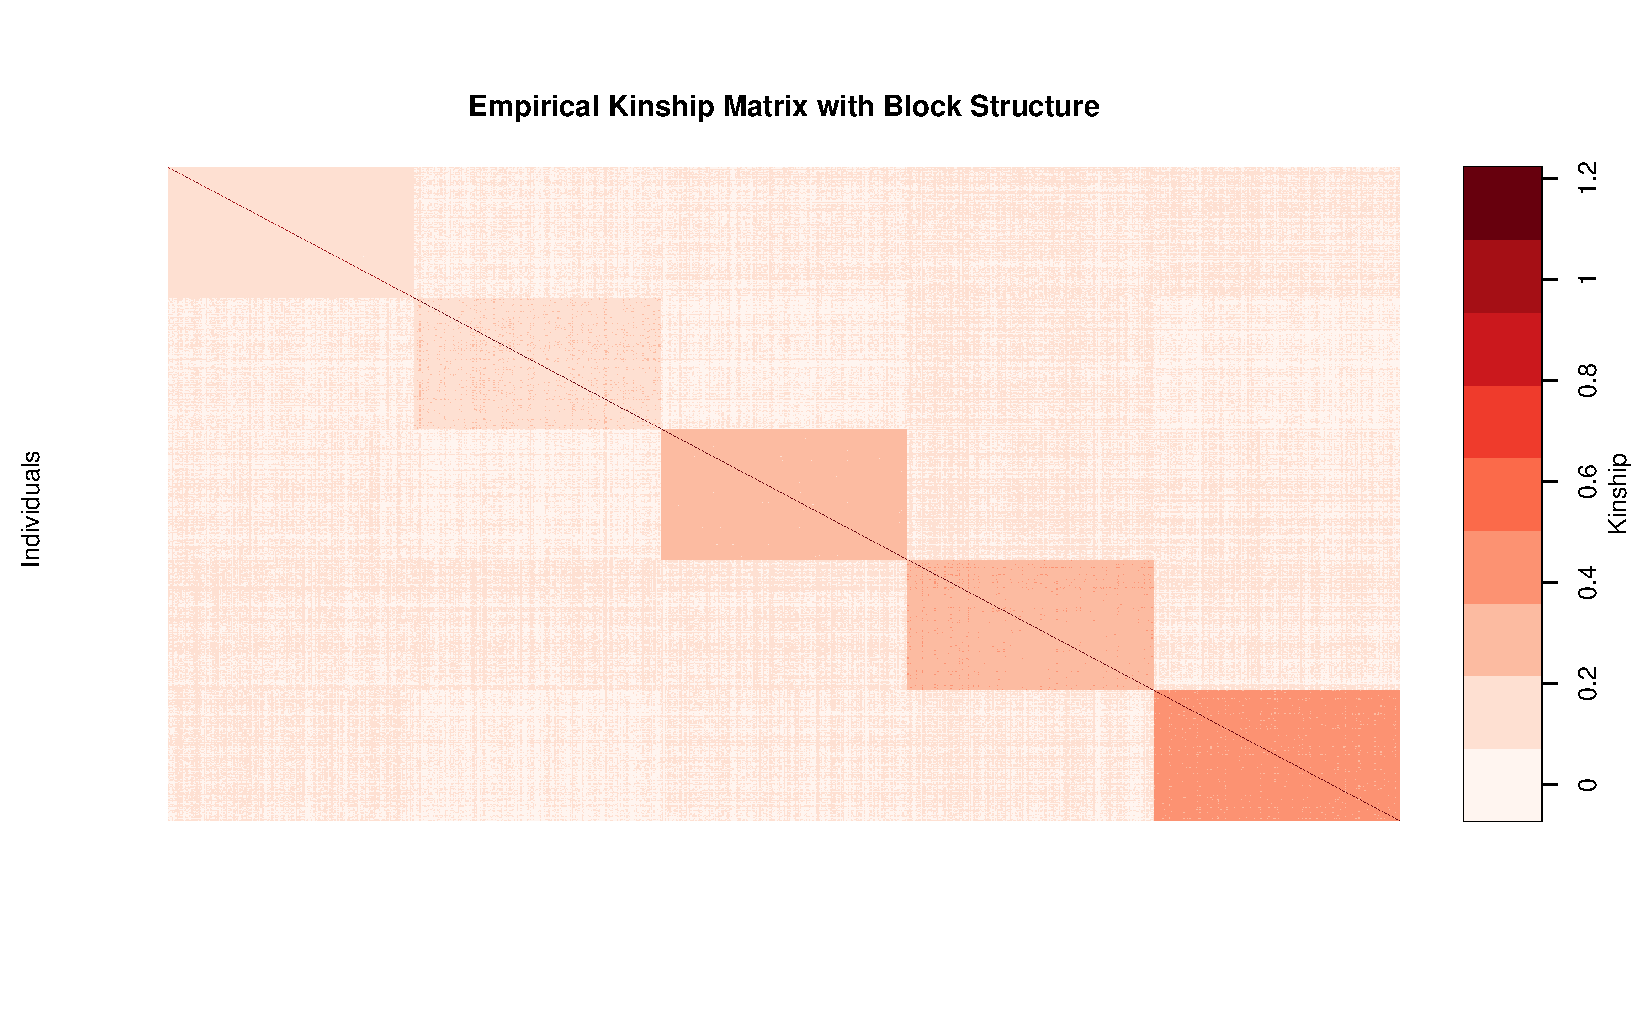
\includegraphics[width=1\linewidth]{figure/plot-kinship-sim-1} 
			
		}
		
		\caption[Empirical kinship matrix with block diagnoal structure used in simulation studies]{Empirical kinship matrix with block diagnoal structure used in simulation studies. Each block represents a subpopulation. }\label{fig:plot-kinship-sim}
	\end{figure}
	
	
\end{knitrout}

In Figure~\ref{fig:plot-pc-sim} we plot the first two principal component scores calculated from the block diagonal kinship matrix in Figure~\ref{fig:plot-kinship-sim}, and color each point by subpopulation membership. We can see that the PCs can identify the subpopulations which is why including them as additional covariates in a regression model has been considered a reasonable approach to control for confounding. 

\begin{knitrout}\scriptsize
	\definecolor{shadecolor}{rgb}{0.969, 0.969, 0.969}\color{fgcolor}\begin{figure}[H]
		
		{\centering 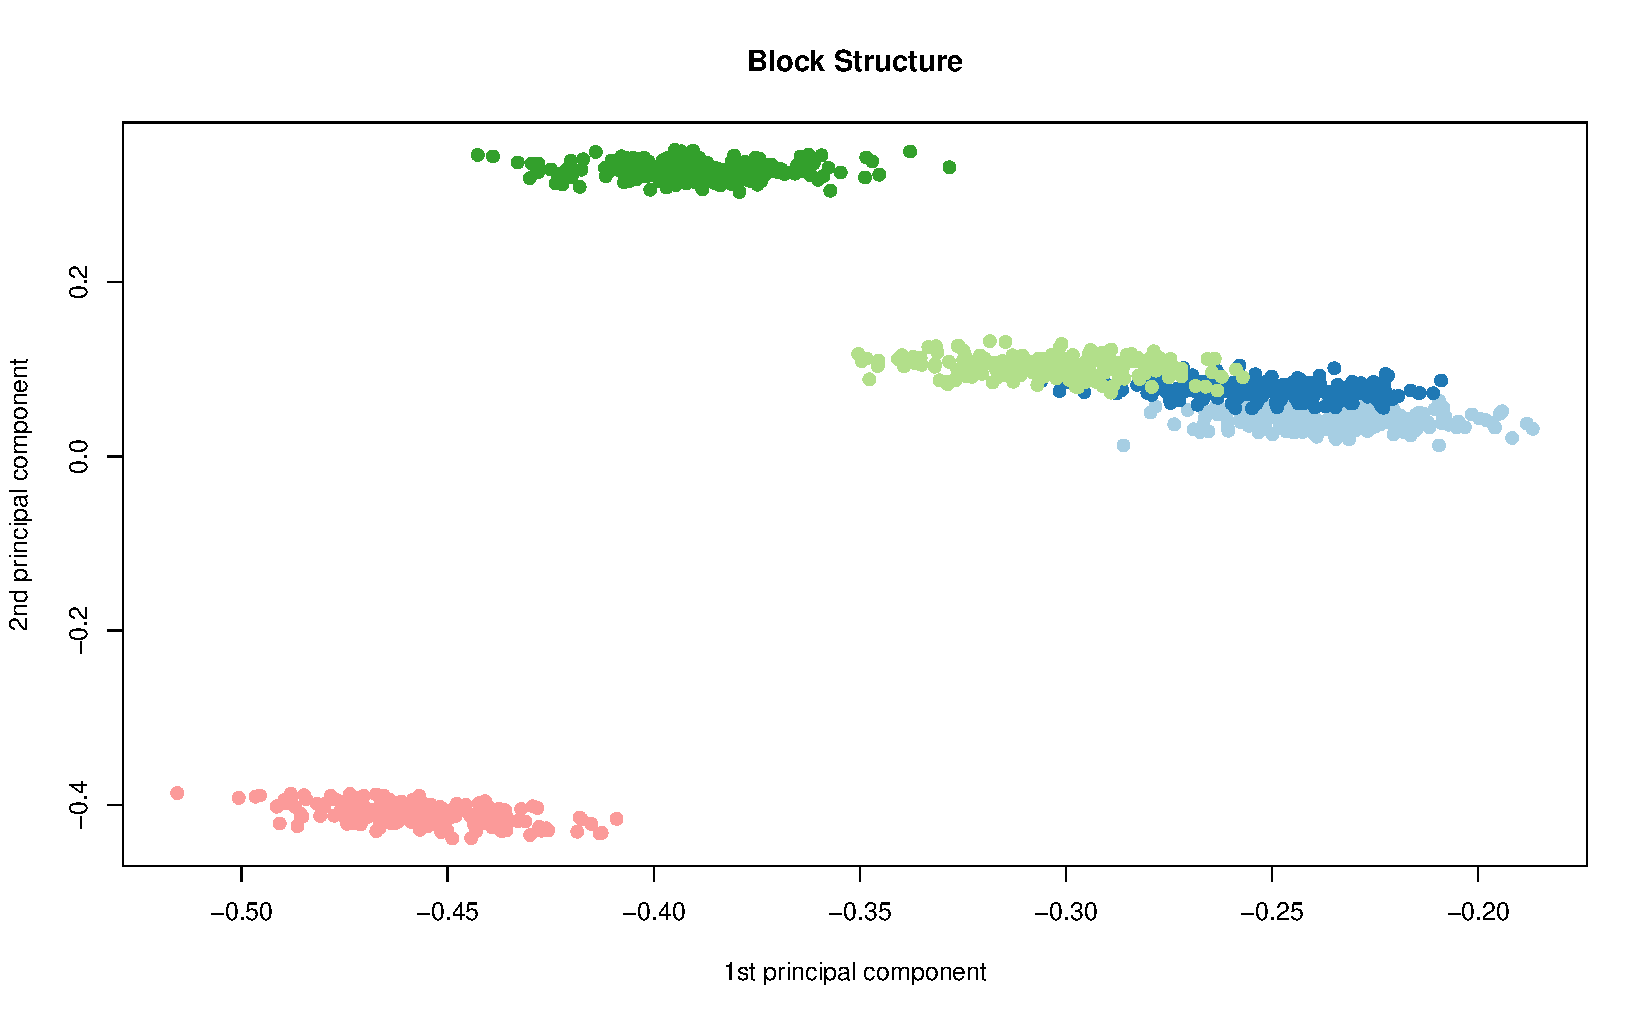
\includegraphics[width=1\linewidth]{figure/plot-pc-sim-1} 
			
		}
		
		\caption[First two principal component scores of the kinship matrix where each color represents one of the 5 simulated subpopulations]{First two principal component scores of the kinship matrix where each color represents one of the 5 simulated subpopulations. The first panel corresponds to 5 independent subpopulations, the second corresponds to a 1 dimensional geographical structure and the thrid panel corresponds to a circular geography.}\label{fig:plot-pc-sim}
	\end{figure}
	
	
\end{knitrout}


For other parameters in our simulation study, we define the following quantities:


\begin{itemize}
	\item $c$: percentage of causal SNPs
	%\item $\rho$: linkage disequilibrium between two SNPs
	\item $\bX^{(fixed)}$: $n \times p_{fixed}$ matrix of SNPs that will be included as fixed effects in our model.
	\item $\bX^{(causal)}$: $n \times (c*p_{fixed})$ matrix of SNPs that will be truly associated with the simulated phenotype, where $\bX^{(causal)} \subseteq \bX^{(fixed)}$
	\item $\bX^{(other)}$: $n \times p_{other}$ matrix of SNPs that will be used in the construction of the kinship matrix. Some of these $\bX^{(other)}$ SNPs, in conjunction with some of the SNPs in $\bX^{(test)}$ will be used in construction of the kinship matrix. We will alter the balance between these two contributors and with the proportion of causal SNPs used to calculate kinship. 
	\item $\bX^{(kinship)}$: $n \times k$ matrix of SNPs used to construct the kinship matrix.
	\item $\beta_j$: effect size for the $j^{th}$ SNP, simulated from a $Uniform(0.3,0.7)$ distribution for $j = 1, \ldots, (c*p_{fixed})$
	%\item $Y^* = \sum_{j=1}^{c*1000} \beta_j \bX^{(causal)}_j$
	%\item $Y = Y^* + k \cdot \varepsilon$, where the error term $\varepsilon$ is generated from a standard normal distribution, and $k$ is chosen such that the signal-to-noise ratio $SNR =\left(Var(Y^*)/Var(\varepsilon)\right)$ is 1
\end{itemize}

We simulate data from the model 
\begin{equation}
\bY = \bX^{(fixed)} \bbeta + \mathbf{P} + \be
\end{equation}
where $\mathbf{P}\sim \mathcal{N}(0, \eta \sigma^2 \bPhi)$ and $\be \sim \mathcal{N}(0, (1-\eta) \sigma^2 \bI)$. The values of the parameters that we used were as follows: narrow sense heritability $\eta=\lbrace 0.1, 0.5 \rbrace$, sample size $n=1000$, number of fixed effects $p_{fixed} = 5000$, number of SNPs used to calculate the kinship matrix $k = 10000$, percentage of causal SNPs $c=\lbrace 0\%, 1\%\rbrace$ and $\sigma^2 = 1$. In addition to these parameters, we also varied the amount of overlap between the causal SNPs and the SNPs used to generate the kinship matrix. We considered two main scenarios:
\begin{enumerate}
	\item None of the causal SNPs are included in the calculation of the kinship matrix: $$\bX^{(kinship)} = \left[\bX^{(other)} \right]$$
	\item All the causal SNPs are included in the calculation of the kinship matrix: $$\bX^{(kinship)} = \left[\bX^{(other)} ; \bX^{(causal)}\right].$$
\end{enumerate}
Both kinship matrices are meant to contrast the model behavior when the causal SNPs are included in both the main effects and random effects versus when the causal SNPs are only included in the main effects. 
These scenarios are motivated by the current standard of practice in GWAS where the candidate marker is excluded from the calculation of the kinship matrix~\citep{lippert2011fast}. 
This approach becomes much more difficult to apply in large-scale multivariable models where there is likely to be overlap between the variables in the design matrix and kinship matrix. 

We compare \ggmix ~to the lasso and the twostep method. For the lasso, we include the first 10 principal components of the estimated kinship as unpenalized predictors in the design matrix. For the twostep method, we first fit an intercept only model with a single random effect using the average information restricted maximum likelihood (AIREML) algorithm~\citep{gilmour1995average} as implemented in the \texttt{gaston} R package~\citep{gaston}. The residuals from this model are then used as the response in a regular lasso model. Note that in the twostep method, we have removed the kinship effect in the first step and therefore do not need to make any further adjustments when fitting the penalized model. We fit the lasso using the default settings in the \texttt{glmnet} package~\citep{friedman2010regularization} and select the optimal value of the regularization parameter using 10-fold cross-validation.  

Let $\hat{\lambda}$ be the estimated value of the optimal regularization parameter selected via cross-validation or GIC, $\widehat{\bbeta}_{\hat{\lambda}}$ the estimate of $\bbeta$ at regularization parameter $\hat{\lambda}$, $S_0 = \left\lbrace j; (\bbeta)_j \neq 0 \right\rbrace$ the index of the true active set, $\widehat{S}_{\hat{\lambda}} = \left\lbrace j; (\widehat{\bbeta}_{\hat{\lambda}})_j \neq 0 \right\rbrace$ the index of the set of non-zero estimated coefficients, and $|A|$ the cardinality of set $A$. 	

We evaluate the methods based on correct sparsity defined as $\frac{1}{p} \sum_{j=1}^{p} A_j$, where 
$$A_j = \begin{cases}
1 & \tm{if } (\widehat{\bbeta}_{\hat{\lambda}})_j= (\bbeta)_j = 0\\
1 & \tm{if } (\widehat{\bbeta}_{\hat{\lambda}})_j \neq 0, (\bbeta)_j \neq 0\\
0 & \tm{if } \tm{else}.
\end{cases}$$
We also compare the model error $(\norm*{\mb{X}\bbeta - \mb{X}\widehat{\bbeta}_{\hat{\lambda}}}_2)$, true positive rate ($\sfrac{|\widehat{S}_{\hat{\lambda}} \in  S_0|}{|S_0|}$), false positive rate ($\sfrac{|\widehat{S}_{\hat{\lambda}} \notin S_0|}{|j \notin S_0|}$), and the variance components for the random effect and error term. The following estimator is used for the error variance of the lasso~\citep{reid2016study}:
\begin{equation}
\frac{1}{n - \widehat{S}_{\hat{\lambda}}} \norm{\bY - \bX \widehat{\bbeta}_{\hat{\lambda}}}_2^2
\end{equation}  

\subsection{Results}



We first plot the correct sparsity results for the null model ($c=0$) and the model with 1\% causal SNPs ($c=0.01$) in Figures~\ref{fig:plot-correct-sparsity-sim-null-model} and~\ref{fig:plot-correct-sparsity-sim-1p-causal}, respectively. When the true model has no causal SNPs, we see that \ggmix ~has perfect Type 1 error control across all 200 replications while both the twostep and lasso methods sometimes estimate a model with a large number of false positives. When the true model contains some causal SNPs, \ggmix ~again outperforms the other two methods in terms of correct sparsity. The distribution of $\widehat{S}_{\hat{\lambda}}$ for each of the three methods is shown in Figure~\ref{fig:plot-nactive-sim-null-model} for $c=0$ and Figure~\ref{fig:plot-nactive-sim-1p-causal} for $c=0.01$ of Supplemental Section~\ref{ap:ggmix_sim_results}. 

\begin{knitrout}\scriptsize
	\definecolor{shadecolor}{rgb}{0.969, 0.969, 0.969}\color{fgcolor}\begin{figure}[h]
		
		{\centering 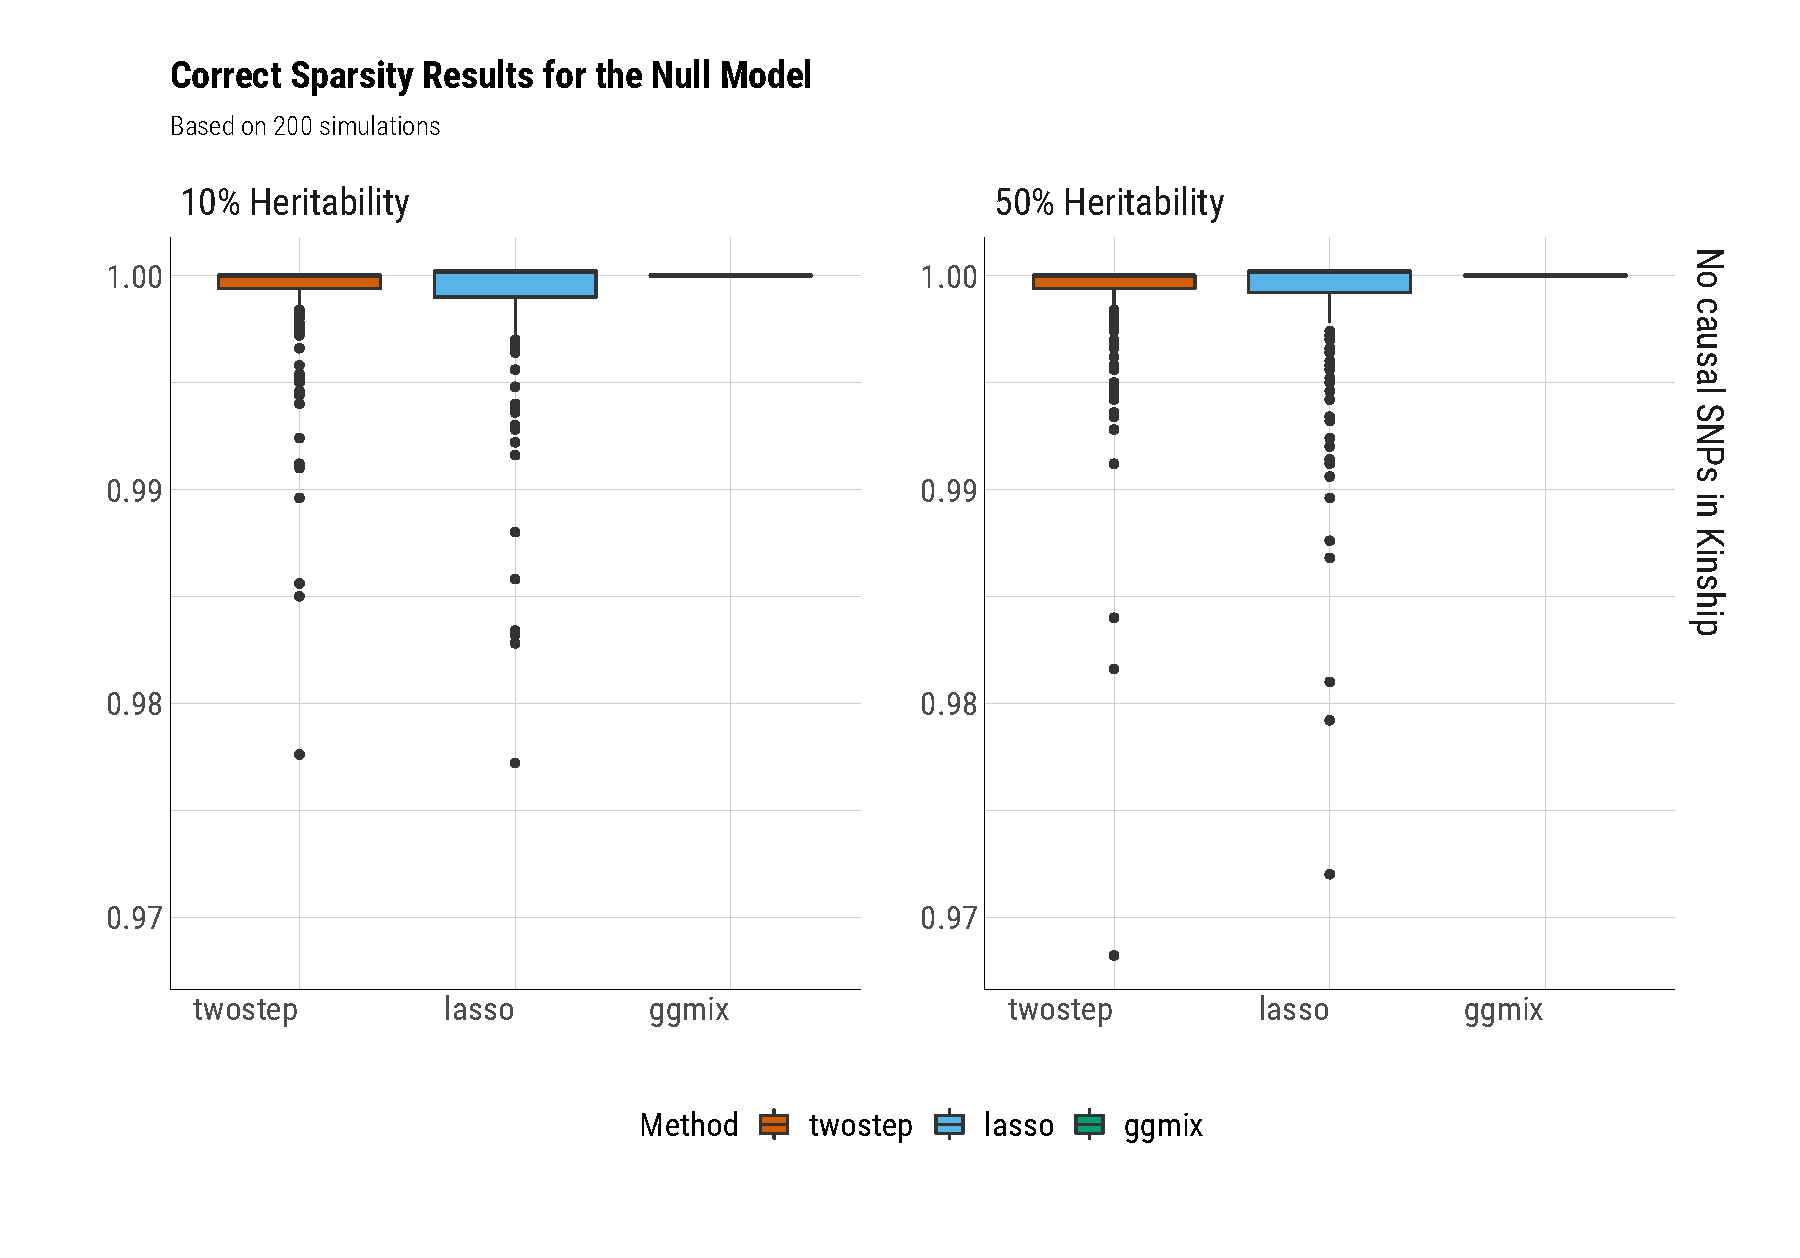
\includegraphics[width=1\linewidth]{figure/plot-correct-sparsity-sim-null-model-1} 
			
		}
		
		\caption[Boxplots of the correct sparsity from 200 simulations by the true heritability $\eta = \lbrace 10\%, 50\% \rbrace$ for the null model ($c=0$)]{Boxplots of the correct sparsity from 200 simulations by the true heritability $\eta = \lbrace 10\%, 50\% \rbrace$ for the null model ($c=0$).}\label{fig:plot-correct-sparsity-sim-null-model}
	\end{figure}
	
	
\end{knitrout}

\begin{knitrout}\scriptsize
	\definecolor{shadecolor}{rgb}{0.969, 0.969, 0.969}\color{fgcolor}\begin{figure}[h]
		
		{\centering 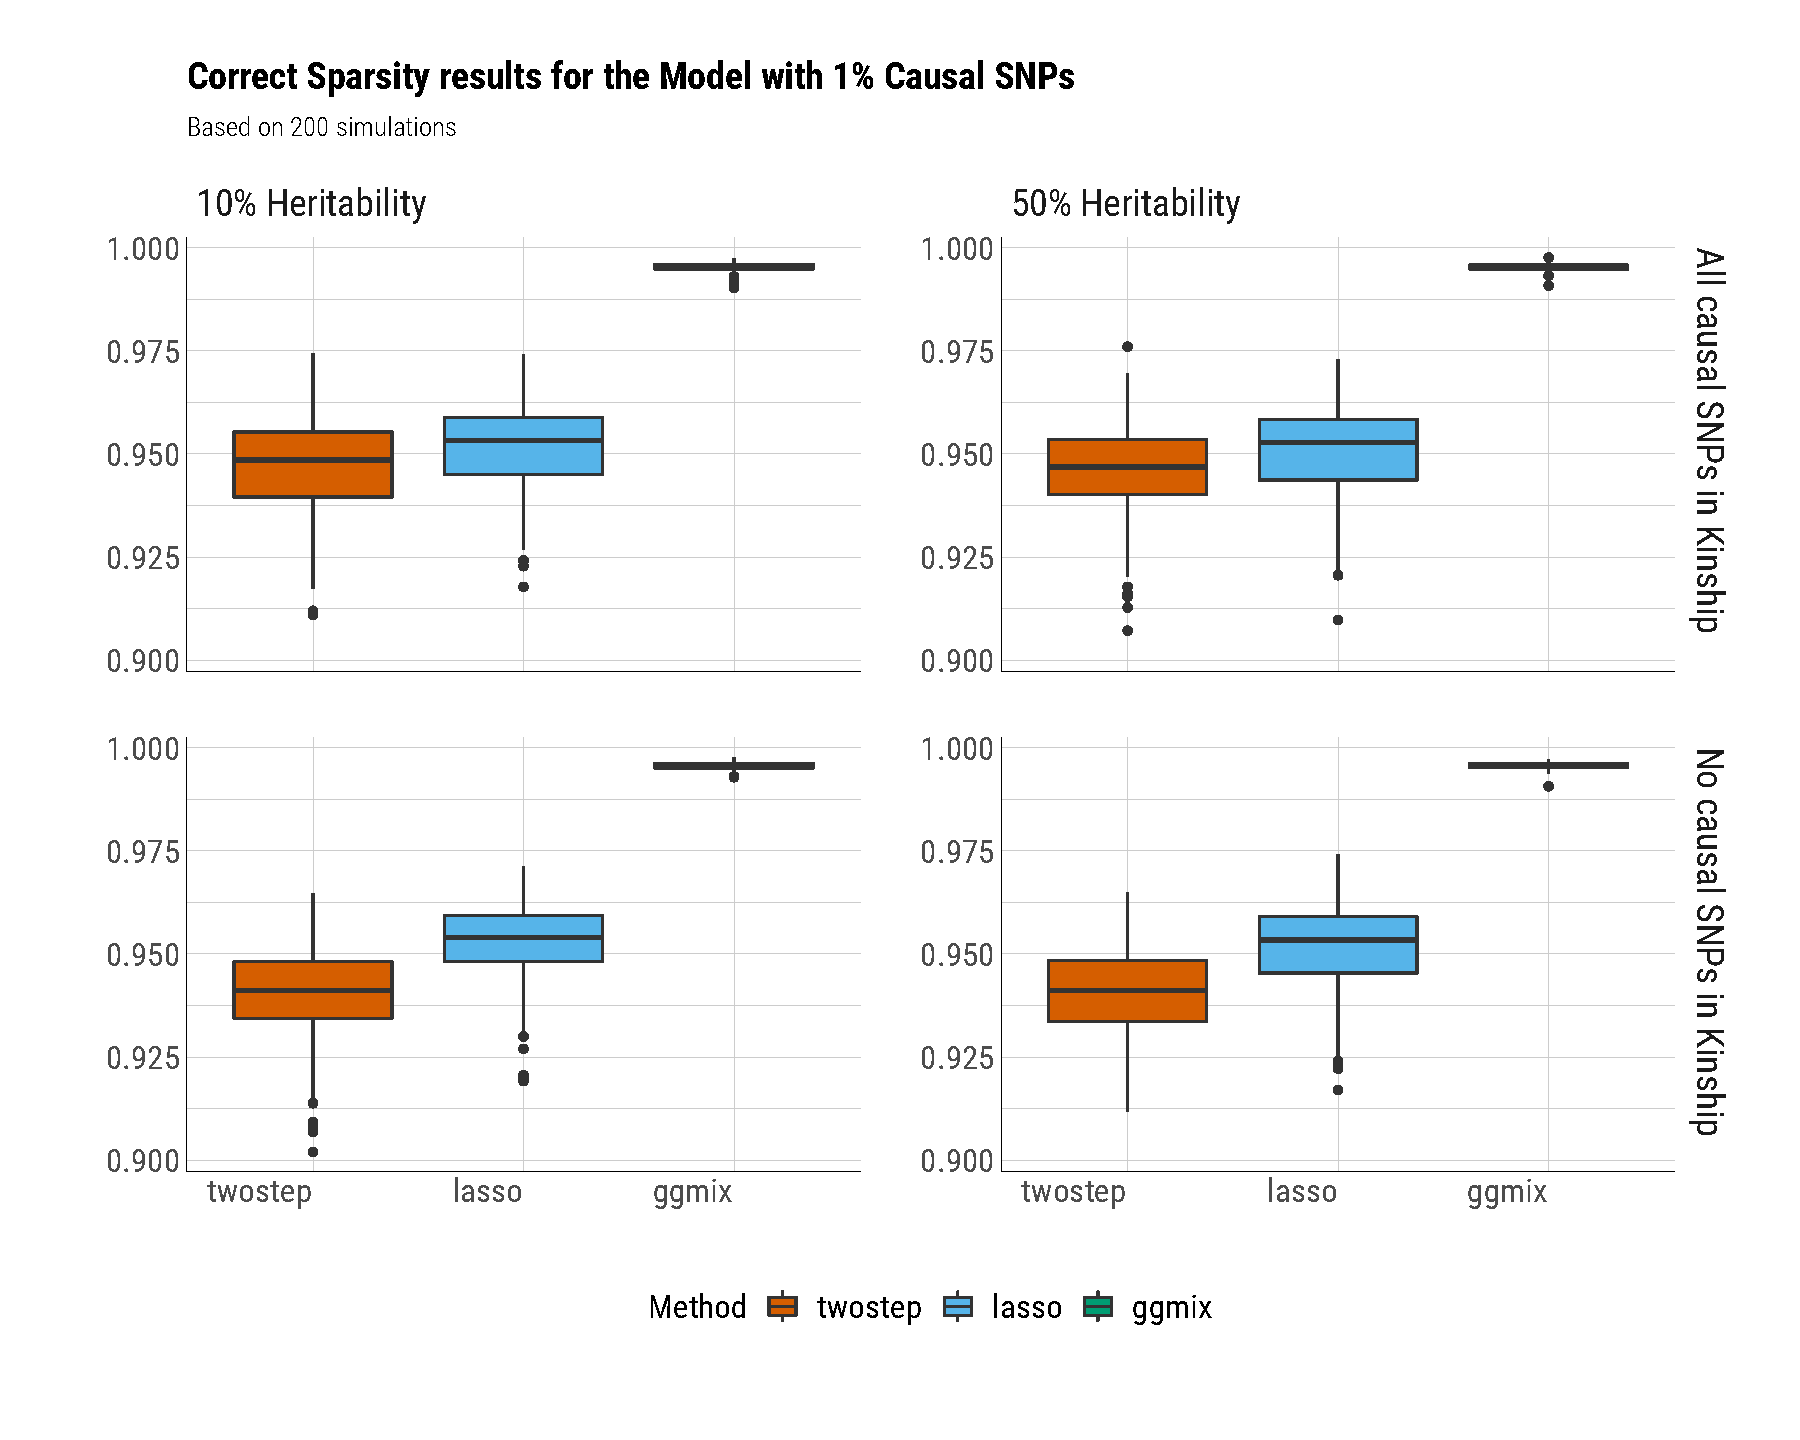
\includegraphics[width=1\linewidth]{figure/plot-correct-sparsity-sim-1p-causal-1} 
			
		}
		
		\caption[Boxplots of the correct sparsity from 200 simulations by the true heritability $\eta = \lbrace 10\%, 50\% \rbrace$ and number of causal SNPs that were included in the calculation of the kinship matrix for the model with 1\% causal SNPs ($c=0.01$)]{Boxplots of the correct sparsity from 200 simulations by the true heritability $\eta = \lbrace 10\%, 50\% \rbrace$ and number of causal SNPs that were included in the calculation of the kinship matrix for the model with 1\% causal SNPs ($c=0.01$).}\label{fig:plot-correct-sparsity-sim-1p-causal}
	\end{figure}
	
	
\end{knitrout}


The true positive vs. false positive rate for the model with 1\% causal SNPs ($c=0.01$) is shown in Figure~\ref{fig:plot-tpr-fpr-sim-1p-causal}. Both the lasso and twostep outperform \ggmix ~in terms of identifying the true model. This accuracy however, comes at the cost of a very high false positive rate compared to \ggmix.

\begin{knitrout}\scriptsize
	\definecolor{shadecolor}{rgb}{0.969, 0.969, 0.969}\color{fgcolor}\begin{figure}[H]
		
		{\centering 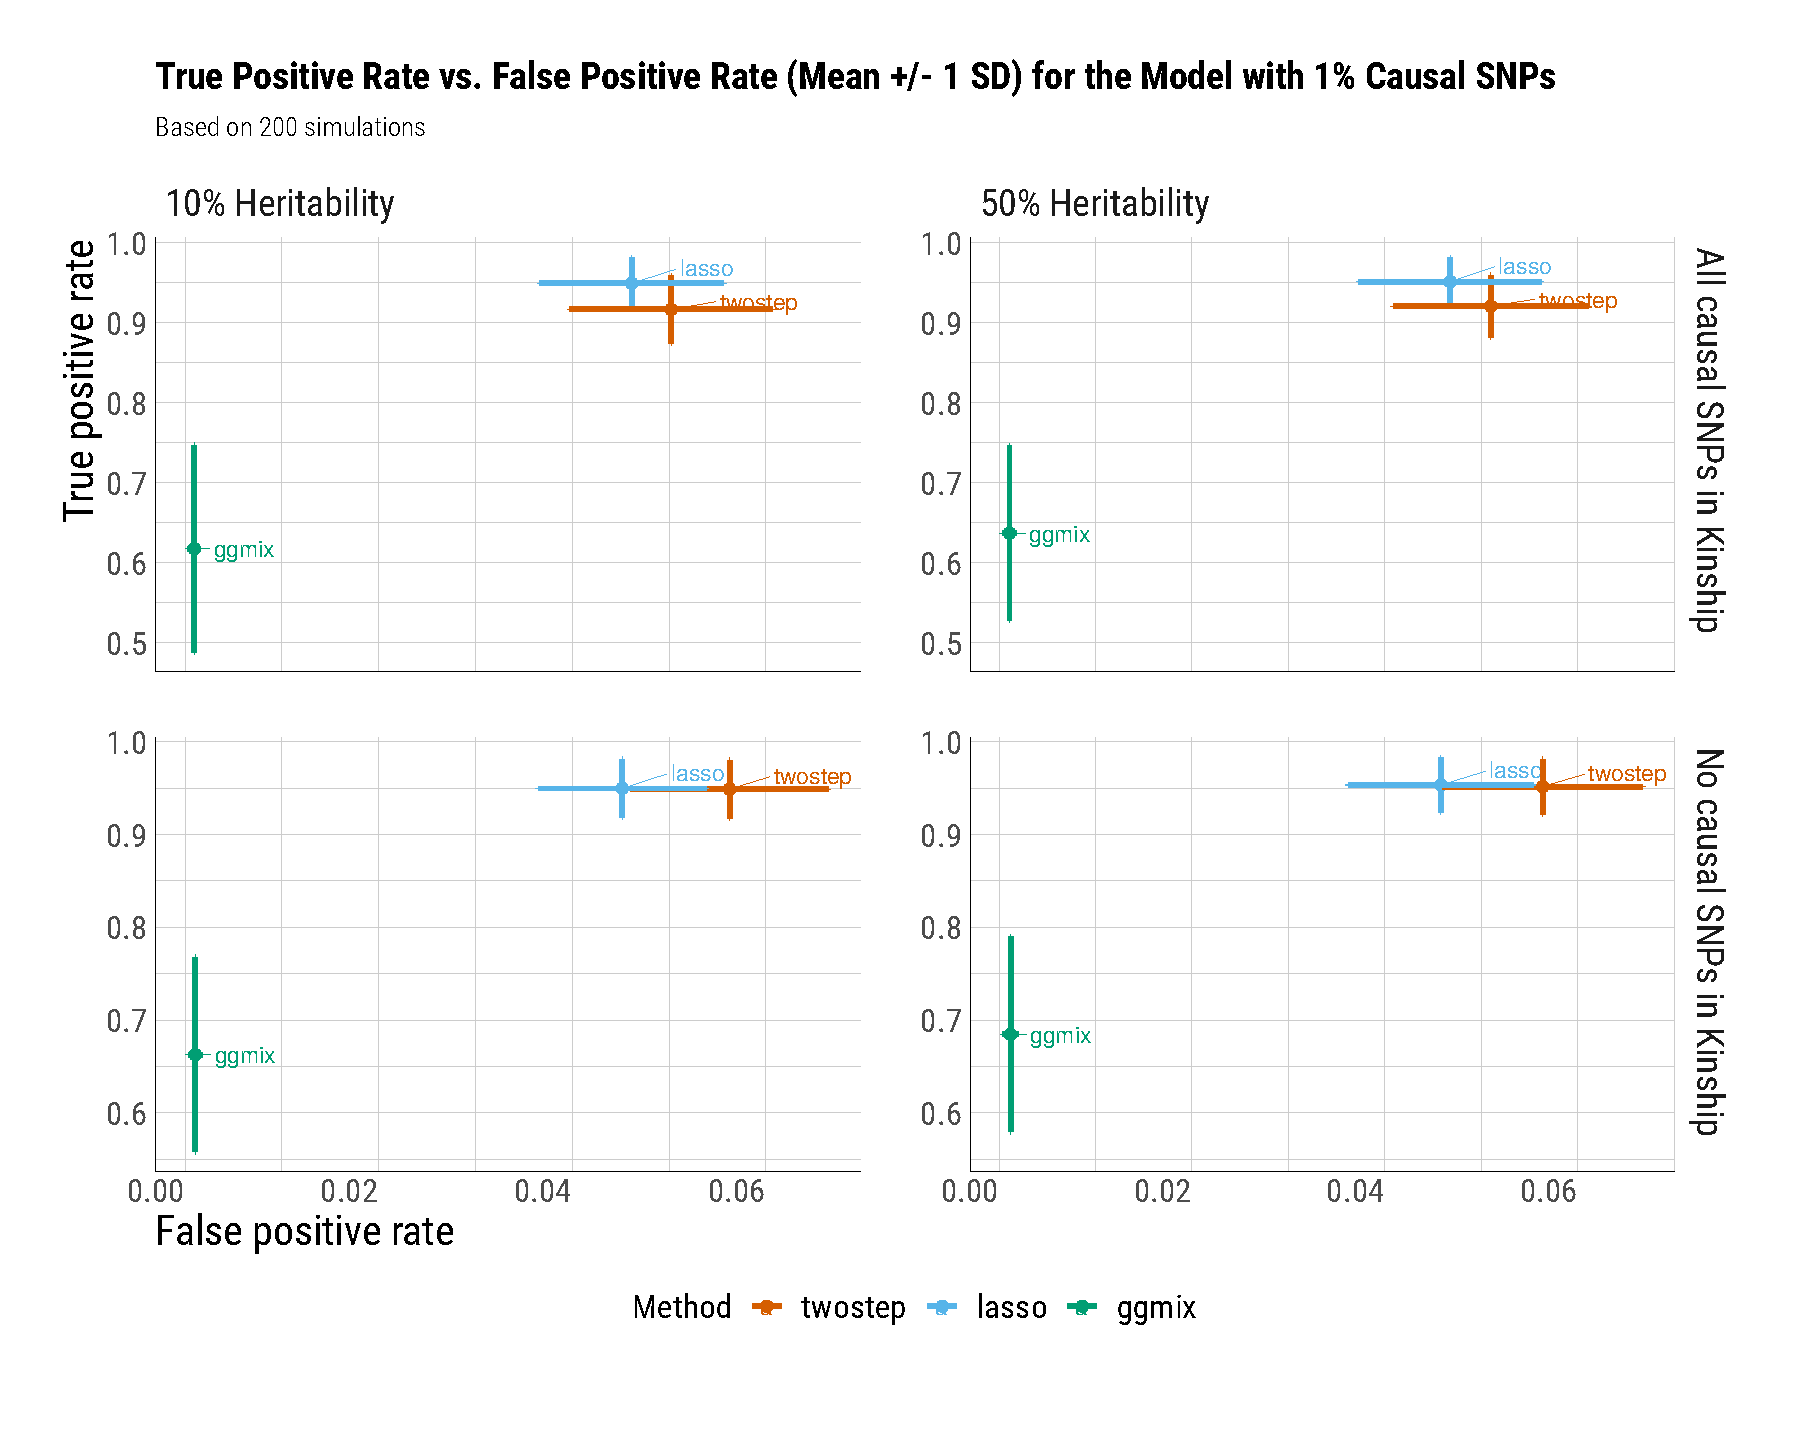
\includegraphics[width=1\linewidth]{figure/plot-tpr-fpr-sim-1p-causal-1} 
			
		}
		
		\caption[Means $\pm 1$ standard deviation of true positive rate vs]{Means $\pm 1$ standard deviation of true positive rate vs. false positive rate from 200 simulations by the true heritability $\eta = \lbrace 10\%, 50\% \rbrace$ and number of causal SNPs that were included in the calculation of the kinship matrix for the model with 1\% causal SNPs ($c=0.01$).}\label{fig:plot-tpr-fpr-sim-1p-causal}
	\end{figure}
	
	
\end{knitrout}

We plot the twostep and \ggmix ~heritability estimates for $c=0$ (Figure~\ref{fig:plot-eta-sim-null-model}, Supplemental Section~\ref{ap:ggmix_sim_results}) and $c=0.01$ (Figure~\ref{fig:plot-eta-sim-1p-causal}). We see that both methods correctly estimate the heritability in the null model. When all of the causal SNPs are in the kinship matrix, both methods overestimate $\eta$ though \ggmix ~is closer to the true value. When none of the causal SNPs are in the kinship, both methods tend to overestimate the truth when $\eta=10\%$ and underestimate when $\eta=50\%$. 

\begin{knitrout}\scriptsize
	\definecolor{shadecolor}{rgb}{0.969, 0.969, 0.969}\color{fgcolor}\begin{figure}[H]
		
		{\centering 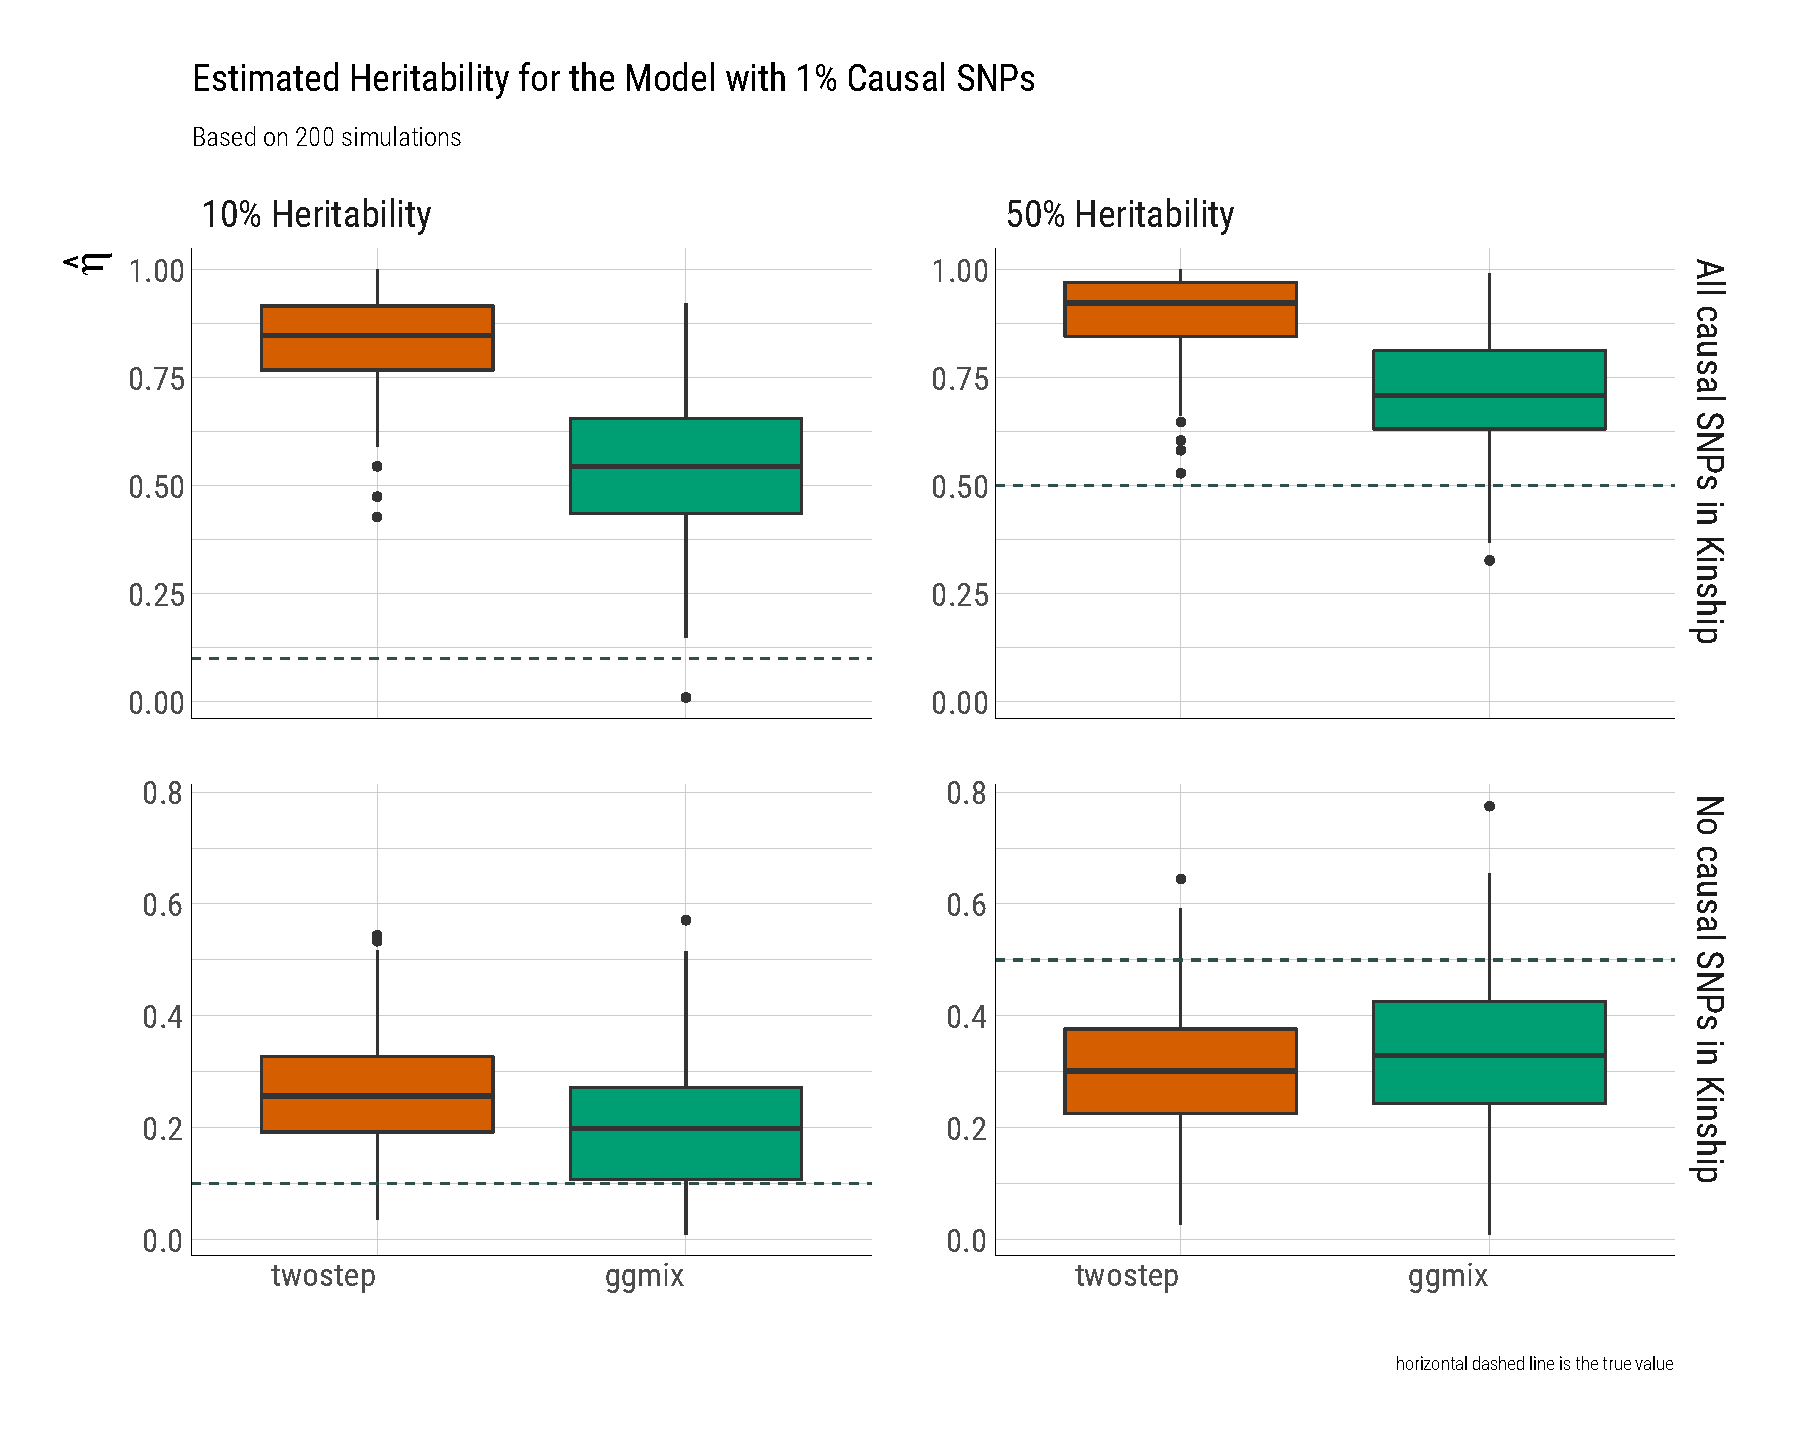
\includegraphics[width=1\linewidth]{figure/plot-eta-sim-1p-causal-1} 
			
		}
		
		\caption[Boxplots of the heritability estimate $\hat{\eta}$ from 200 simulations by the true heritability $\eta = \lbrace 10\%, 50\% \rbrace$ and number of causal SNPs that were included in the calculation of the kinship matrix for the model with 1\% causal SNPs ($c=0.01$)]{Boxplots of the heritability estimate $\hat{\eta}$ from 200 simulations by the true heritability $\eta = \lbrace 10\%, 50\% \rbrace$ and number of causal SNPs that were included in the calculation of the kinship matrix for the model with 1\% causal SNPs ($c=0.01$).}\label{fig:plot-eta-sim-1p-causal}
	\end{figure}
	
	
\end{knitrout}


In Figures~\ref{fig:plot-errorvar-sim-null-model} (Supplemental Section~\ref{ap:ggmix_sim_results}) and~\ref{fig:plot-errorvar-sim-1p-causal}, we plot the error variance for $c=0$ and $c=0.01$, respectively.
The twostep and \ggmix ~methods correctly estimate the error variance while the lasso overestimates it for the null model and for when 1\% of the causal SNPs are in the kinship matrix. We see an inflated estimated error variance across all three methods when $c=0.01$ and none of the causal SNPs are in the kinship matrix with the lasso and \ggmix ~performing similarly. 


\begin{knitrout}\scriptsize
	\definecolor{shadecolor}{rgb}{0.969, 0.969, 0.969}\color{fgcolor}\begin{figure}[H]
		
		{\centering 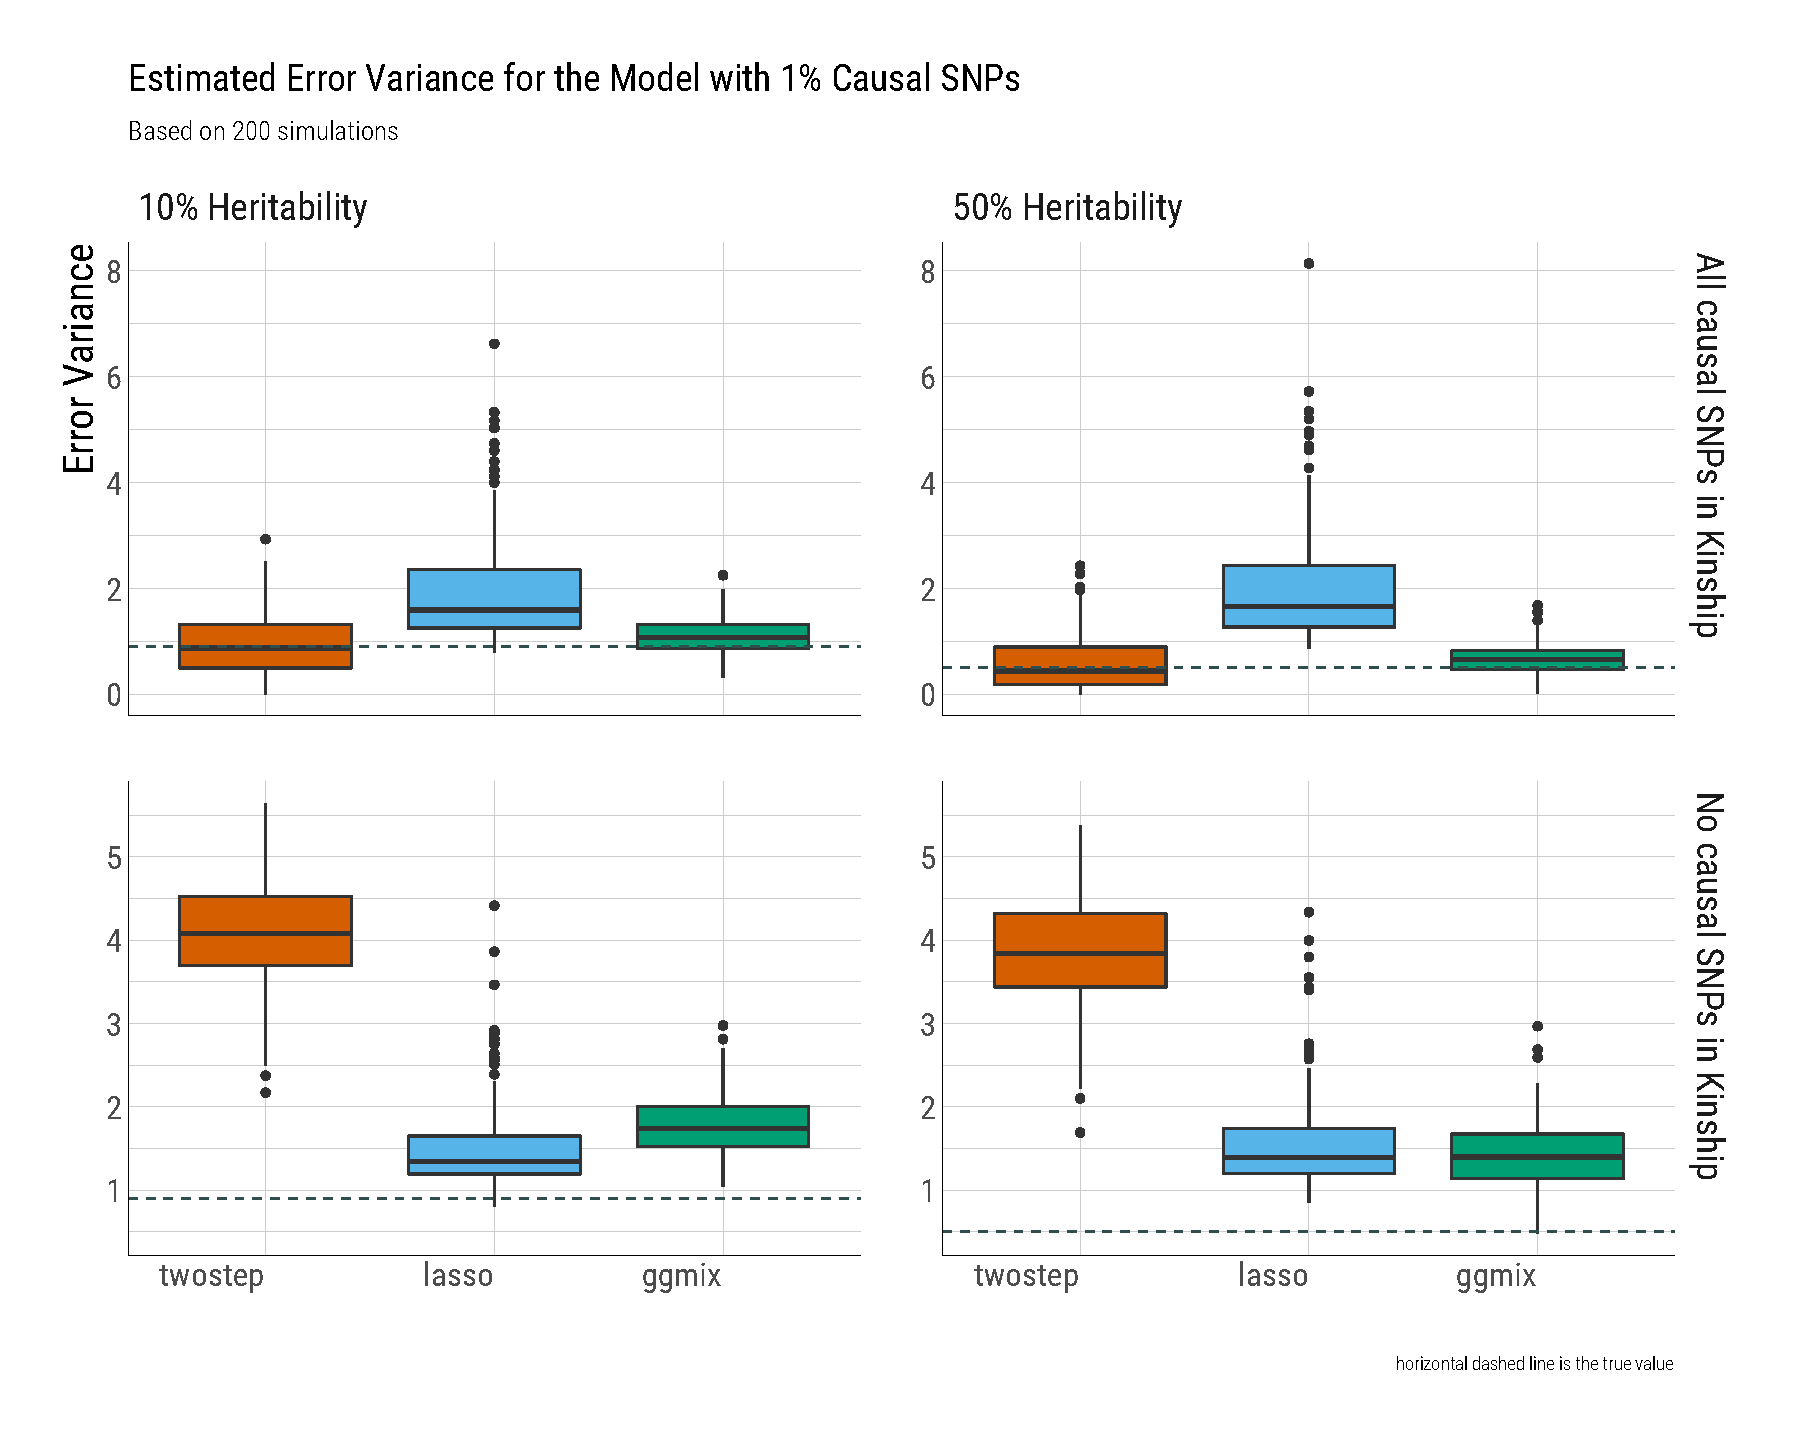
\includegraphics[width=1\linewidth]{figure/plot-errorvar-sim-1p-causal-1} 
			
		}
		
		\caption[Boxplots of the estimated error variance from 200 simulations by the true heritability $\eta = \lbrace 10\%, 50\% \rbrace$ and number of causal SNPs that were included in the calculation of the kinship matrix for the model with 1\% causal SNPs ($c=0.01$)]{Boxplots of the estimated error variance from 200 simulations by the true heritability $\eta = \lbrace 10\%, 50\% \rbrace$ and number of causal SNPs that were included in the calculation of the kinship matrix for the model with 1\% causal SNPs ($c=0.01$).}\label{fig:plot-errorvar-sim-1p-causal}
	\end{figure}
	
	
\end{knitrout}


We compare the model error as a function of $\widehat{S}_{\hat{\lambda}}$ in Figures~\ref{fig:plot-me-nactive-sim-null} (Supplemental Section~\ref{ap:ggmix_sim_results}) and~\ref{fig:plot-me-nactive-sim-1p-causal} for $c=0$ and $c=0.01$, respectively. Lasso achieves the smallest model error across all scenarios (for $c=0.01$), albeit with a large number of active variables. \ggmix ~has a smaller model error compared to twostep when all causal SNPs are in the kinship matrix and similar performance when none of the causal SNPs are in the kinship matrix. 

\begin{knitrout}\scriptsize
	\definecolor{shadecolor}{rgb}{0.969, 0.969, 0.969}\color{fgcolor}\begin{figure}[H]
		
		{\centering 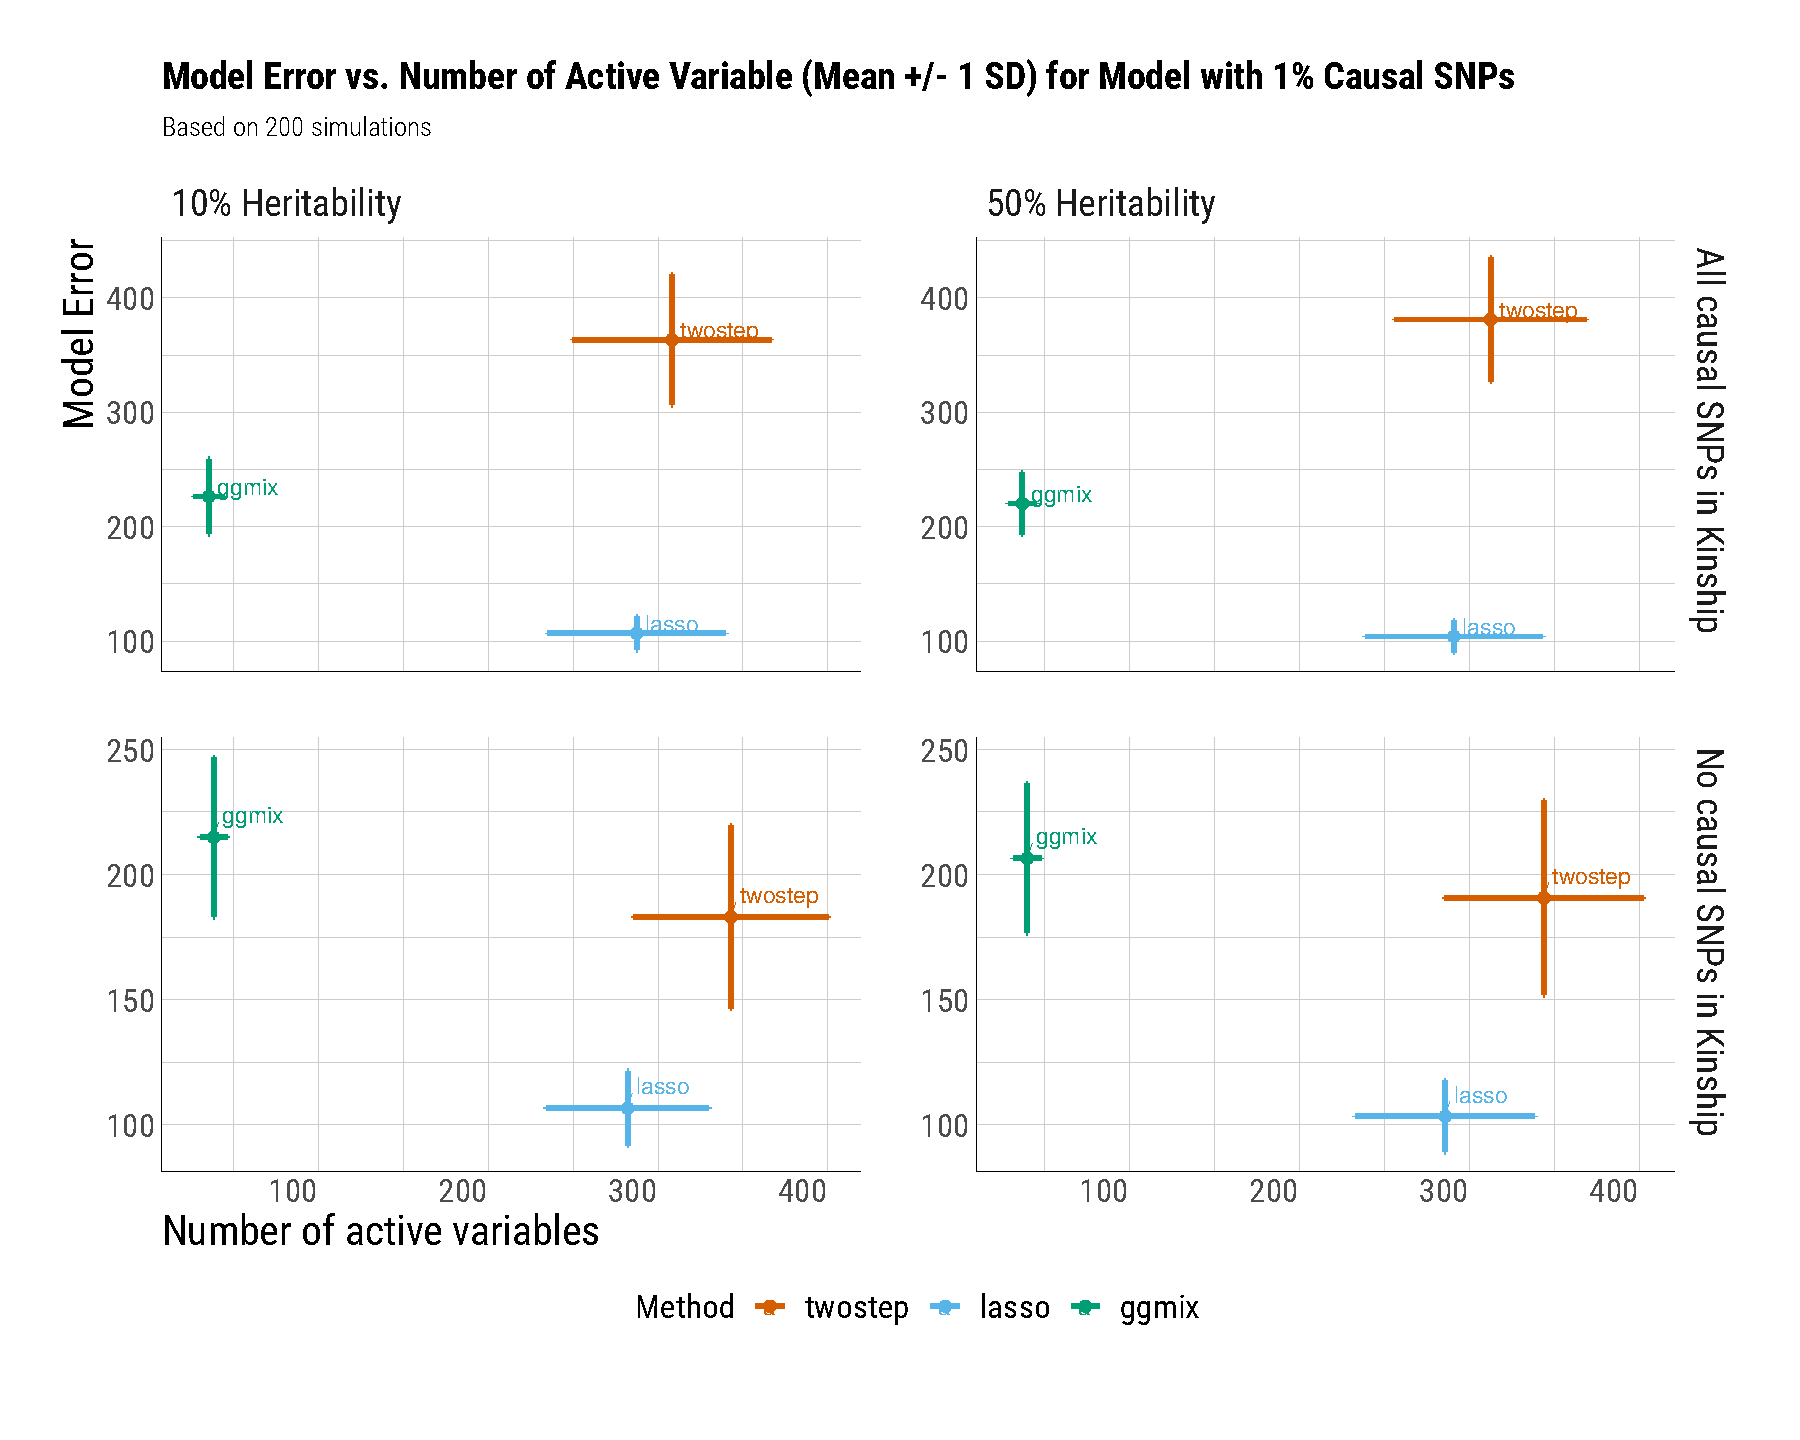
\includegraphics[width=1\linewidth]{figure/plot-me-nactive-sim-1p-causal-1} 
			
		}
		
		\caption[Means $\pm 1$ standard deviation of the model error vs]{Means $\pm 1$ standard deviation of the model error vs. the number of active variables by the true heritability $\eta = \lbrace 10\%, 50\% \rbrace$ and number of causal SNPs that were included in the calculation of the kinship matrix for the model with 1\% causal SNPs ($c=0.01$).}\label{fig:plot-me-nactive-sim-1p-causal}
	\end{figure}
	
	
\end{knitrout}

Overall, we observe that variable selection results for \ggmix ~are similar regardless of whether the causal SNPs are in the kinship matrix or not. 
This result is encouraging since in practice the kinship matrix is constructed from a random sample of SNPs across the genome, some of which are likely to be causal. 
\ggmix ~has very good Type 1 error control, while both the lasso and twostep have a very high false positive rate. 
Inclusion of the causal SNPs in the kinship calculation has a strong impact on the variance component estimation with the heritabilty and error variance estimates working in opposite directions. 
That is, when all causal SNPs are in the kinship matrix, the heritability estimates are biased towards 1 while the error variance is correctly estimated. 
Conversely, when none of the causal SNPs are included in the kinship matrix, the estimated heritability is closer to the true value, while the error variance is inflated. 
Both the lasso and twostep methods have better signal recovery as compared to \ggmix. 
However, this signal is being spread across many variables leading to many Type 1 errors. 

\section{Discussion}

We develop a general penalized LMM framework for population structure correction that simultaneously selects and estimates variables, accounting for between individual correlations, in one step. 
Our CGD algorithm is computationally efficient and has theoretical guarantees of convergence. 
We provide an easy-to-use software implementation of our algorithm along with a principled method for automatic tuning parameter selection. 
Through simulation studies, we show that existing approaches such as a two-stage approach or the lasso with a principal component adjustment lead to a large number of false positives.     
Our proposed method has excellent Type 1 error control and is robust to the inclusion of causal SNPs in the kinship matrix. This feature is important since in practice the kinship matrix is constructed from a random sample of SNPs across the genome, some of which are likely to be causal. 

Although we derive a CGD algorithm for the $\ell_1$ penalty, our approach can also be easily extended to other penalties such as the elastic net and group lasso with the same guarantees of convergence. 

%To our knowledge, we are the first to develop a CGD algorithm in the specific context of fitting a penalized LMM for population structure correction with theoretical guarantees of convergence. Furthermore, we develop a principled method for automatic tuning parameter selection and provide an easy-to-use software implementation in order to promote wider uptake of these more complex methods by applied practitioners.   

A limitation of \ggmix ~is that it first requires computing the covariance matrix with a computation time of $\mathcal{O}(n^2k)$ followed by a spectral decomposition of this matrix in $\mathcal{O}(n^3)$ time where $k$ is the number of SNP genotypes used to construct the covariance matrix. This computation becomes prohibitive for large cohorts such as the UK Biobank~\citep{allen2012uk} which have collected genetic information on half a million individuals. When the matrix of genotypes used to construct the covariance matrix is low rank, there are additional computational speedups that can be implemented. While this has been developed for the univariate case~\citep{lippert2011fast}, to our knowledge, this has not been explored in the multivariable case. We are currently developing a low rank version of the penalized LMM developed here, which reduces the time complexity from $\mathcal{O}(n^2k)$ to $\mathcal{O}(nk^2)$.

%There is thus a need to develop newer methodologies that reflect the increasing size and genetic heterogeneity of the large cohort studies being assembled today.  



%The LMM-lasso paper mentions that this is possible but does not provide further details on how this can be implemented in a penalized mixed model framework. 
While the predominant motivation for our approach has been association testing, we believe that there are other applications in which it can be used as well. 
For example, in the most recent Genetic Analysis Workship 20 (GAW20),  the causal modeling group investigated causal
relationships between DNA methylation (exposure) within some genes
and the change in high-density lipoproteins $\Delta$HDL (outcome) using Mendelian randomization (MR)~\citep{davey2003mendelian}. 
Penalized regression methods could be used to select SNPs strongly associated with the exposure in order to be used as an instrumental variable (IV). 
However, since GAW20 data consisted of families, two step methods were used which could have resulted in a large number of false positives. \ggmix~is an alternative approach that could be used for selecting the IV while accounting for the familial structure of the data. 
Our method is also suitable for fine mapping SNP association signals in genomic regions, where the goal is to pinpoint individual variants most likely to impact the undelying biological mechanisms of disease~\citep{spain2015strategies}.
